\chapter{Approach And Methods} % Chapter title

\label{chapter:approach_and_methods} % For referencing the chapter elsewhere, use \ref{chapter:computational_neuro} 

\def \blochwidth {0.3}
%\newcommand{\crzgate}{$\mathrm{CR_Z}$}
\newcommand{\plani}{$\mathcal{P}_i$}
\newcommand{\planj}{$\mathcal{P}_j$}
\newcommand{\querya}{$\mathcal{Q}_a$}
\newcommand{\queryb}{$\mathcal{Q}_b$}

% table cell head
\renewcommand{\cellalign}{lc}
\renewcommand{\theadalign}{cc}
\renewcommand\theadgape{\Gape[4pt]}
\renewcommand\theadfont{\normalsize}
\renewcommand\cellgape{\Gape[5pt]}
\renewcommand*{\arraystretch}{1.2}
%---------------------------------------------------------------------------------------

\section{Quantum Neural Network}
\label{chapter:approach_methods_qnn}

\subsection{Datasets and Data Acquisition}
\label{subsection:qnn_datasets_and_acqusition}
To allow a direct comparison to the QSVM results achieved by Smailov et al.\cite{smailovQuantumMachineLearning2021}, the same binary datasets are used which are shown in table \ref{table:qnn_binary_datasets}.

\begin{table}[!h]
	\centering
	\begin{tabular}{rccc}
		\hline 
		\thead{\textbf{Dataset}} & \thead{\textbf{\#Features}} & \thead{\textbf{\#Records}} & \thead{\textbf{\#Classes}} \\
		\hline 
		Adhoc   & 3         & 100      & 2        \\
		Custom  & 2         & 100      & 2        \\
		Iris    & 4         & 100      & 2        \\
		Rain    & 5         & 100      & 2        \\
		Vlds    & 5         & 100      & 2        \\
		\hline
	\end{tabular}
	\caption{Characteristics of the five binary datasets used in our first QNN experiments.}
	\label{table:qnn_binary_datasets}
\end{table}

The dataset choice by itself has some problems that have to be addressed. To begin with, they are all binary, as well as quite limited in the number of total avaliable records that can be used to train and evaluate. Table \ref{table:qnn_extended_datasets} shows the extended dataset used in this thesis to do the same evaluation using quantum neural networks. The datasets use more records when possible. In addition, the \emph{Iris} dataset is used with all three classes instead of only two. Due to the current limitation when it comes to using real hardware, as well as the design choice of using a qubit per feature, the circuit designs are limited to a maximum of five qubits. This is further explained in chapter \ref{subsection:limitations_and_shortcomings}. In the case of the \emph{Rain} dataset, principal component analysis, or PCA\footnote{A detailed explanation on what PCA is and how it works can be found here \cite{bro2014principal}} in short, was used to determine 5 features to encode.

\begin{table}[!h]
	\centering
	\begin{tabular}{rcccc}
		\hline 
		\thead{\textbf{Dataset}} & \thead{\textbf{\#Features}} & \thead{\textbf{\#Records}} & \thead{\textbf{\#Classes}} & \thead{\textbf{PCA}} \\
		\hline 
		Adhoc   & 3         & 1000      & 2          & no        \\
		Custom  & 2         & 1000      & 2          & no        \\
		Iris    & 4         & 150       & 3          & no        \\
		Rain    & 5         & 1000      & 2          & yes       \\
		Vlds    & 5         & 1000      & 2          & no        \\
		\hline
	\end{tabular}
	\caption{Characteristics of the five extended datasets used in our second QNN experiments. The row PCA denotes if the features were selected using PCA or not.}
	\label{table:qnn_extended_datasets}
\end{table}

\clearpage

\subsubsection{Datasets}

\textbf{Iris}\\ 
This is a well known and widely used dataset. It is loaded via the \code{load\_iris} function from scikit-learn \cite{SklearnDatasetsLoad}. For the binary dataset, 100 records and two classes are used, whilst for the extended dataset all 150 records and 3 classes are used.
\\
\\
\textbf{Rain}\\
This dataset contains roughly 10 years of daily weather observations from many locations across Australia. It is a binary dataset where the goal is the prediction of rain on the following day, denoted by the attribute \textit{RainTomorrow}. Incomplete data entries of this set are dropped and a balanced subsampling performed. For the initial experiments with the normal datasets, the same features are selected as by Smailov et al., namely \textit{MinTemp}, \textit{Humidity9am}, \textit{WindSpeed3pm}, \textit{Pressure9am}, \textit{WindDir9am}. The second experiment with the extended datasets uses PCA to select the five features.
\\
\\
\textbf{Adhoc}\\
This dataset is generated using the \code{ad\_hoc\_data} from \code{qiskit}\cite{AdHocData}, which itself is based on the work of Havlicek et al.\cite{havlicekSupervisedLearningQuantum2019}
\\
\\
\textbf{Vlds}\\
A random multi-label classification problem, generated using the\\ \code{make\_multilabel\_classification} function from scikit-learn\cite{scikit-learn}.
\\
\\
\textbf{Custom}\\
A binary two feature dataset generated by a custom algorithm using the \code{numpy.random.default rng} function. Figure \ref{figure:custom_dataset} plots the two avaliable labels $0.0$ and $1.0$. As shown, $1.0$ is distributed in a square shape, whilst $0.0$ is distributed along the diagonals of said shape.

\begin{figure}[!ht]
    \centering
    \scalebox{0.9}{
        \includegraphics[width=0.66\linewidth]{thesis/Figures/qnn/custom_dataset.png}
    }
    \caption{Custom dataset which needs a higher-order function to classify the data points. Source: \cite{smailovQuantumMachineLearning2021}}
    \label{figure:custom_dataset}
\end{figure}

\subsubsection{Preprocessing}
All the previously mentioned datasets are normalized and scaled using scikit-learns\cite{scikit-learn} \code{StandardScaler} and \code{MinMaxScaler} - with a target range of $[-1, 1]$. This normalization and scaling is adopted from the work of Smailov et al.\cite{smailovQuantumMachineLearning2021}.\par
A crucial preprocessing step is the mapping of the targets to integer values starting from $0$. For example, $0$ denotes the first class, $1$ the second one etc. This is necessary so that the parity function, shown in listing \ref{listing:parity_function}, can compare its prediction to our targets. \par
For training and testing, the data is split into two subsets. The training set is made out of $80$\% of the original dataset, with the remaining $20$\% used for the testing set. Each training iteration is done 10 times, with each of these 10 runs featuring a randomly shuffled training and testing set.

\subsection{Variational Quantum Algorithm Classifier} 
The classification is a standard problem in machine learning which can be solved by using supervised learning. For this, a set of features $\mathcal{X}$, a set of labels $\mathcal{Y}$, as well as a pairwise dataset $\mathcal{D} = \{(x^1,y^1),...,(x^M,y^M)\}$ with $x^m \in \mathcal{X}$ and $y^m \in \mathcal{Y}$ for $m= 1,..,M$ is needed. The goal is to predict $y \in \mathcal{Y}$ from a feature $x^m \in \mathcal{X}$. For binary classification, the following is assumed: $\mathcal{X} = \mathbb{R}^N$ and $\mathcal{Y} = \{0,1\}$. In the case of multi-label classification $\mathcal{Y} = \{0,1,...,c\}$, where $c$ is the total number of labels and a $N$-dimensional real feature space is assumed.\par
In a first step, the quantum circuit $f(x,\theta)$ is trained with the input features by adjusting the parameters $\theta$, which will be called weights from this point on. The evaluation is done using the trained weights to predict $y$.\par
For the supervised training runs to optimize their weights, a VQA based hybrid classical-quantum approach is used, as previously described in chapter \ref{subsection:vqa_fundamentals}. Training a quantum model means to find the measurement which minimises a cost function that depends on training data. To achieve this,  the two \code{qiskit}\cite{Qiskit} classes \code{CircuitQNN} and \code{NeuralNetworkClassifier} are used to build a neural network classifier from a given variational quantum circuit as seen in code listing \ref{listing:qnn_network_classifier_python}. The \code{squared\_error} L2 loss function used by \code{NeuralNetworkClassifier} as the default loss function can be seen in equation \ref{equation:l2loss}.

\begin{equation}
    \centering
        L2Loss = \sum _{i=1}^n\left(y_{true}-y_{predicted}\right)^2
    \label{equation:l2loss}
\end{equation}

\begin{listing}[!h]
    \begin{minted}[linenos,fontsize=\scriptsize]{python}
from qiskit.utils import QuantumInstance
from qiskit_machine_learning.neural_networks import CircuitQNN
from qiskit_machine_learning.algorithms.classifiers import NeuralNetworkClassifier

quantum_instance = QuantumInstance(q_simulator, shots=1024)

circuit_qnn = CircuitQNN(circuit=circuit,
                         input_params=circuit.parameters[-n_features:],
                         weight_params=circuit.parameters[:-n_features],
                         interpret=parity,
                         output_shape=output_shape,
                         quantum_instance=quantum_instance)

# construct classifier
return NeuralNetworkClassifier(neural_network=circuit_qnn,
                               callback=callback,
                               optimizer=optimizer[0])
    \end{minted}
    \caption{Python code snippet to create a \code{NeuralNetworkClassifier} from a given quantum circuit used in the experiments for training.}
    \label{listing:qnn_network_classifier_python}
\end{listing}

\subsubsection{Parity function}
\label{subsubsection:parity_function_explained}
To determine the resulting \textit{label} of a measurement, as example shown in figure \ref{figure:parity_function_example_histogram}, the \code{parity} function described in listing \ref{listing:parity_function} is given as argument for the interpret parameter of the \code{CircuitQNN} class. This can be seen in detail in listing \ref{listing:qnn_network_classifier_python} on line number $10$. 

\begin{figure}[!h]
    \centering
    \scalebox{1}{
        \includegraphics[width=0.66\linewidth]{thesis/Figures/qnn/qiskit_simulator_run_parity_histogram.png} 
    }
    \caption{Histogram of the results after measuring an arbitrary quantum circuit with two qubits. The \code{python} object behind the data is a dictionary with the format \code{\{'00': 383, '01': 1022, '10': 2501, '11': 94\}}.}
    \label{figure:parity_function_example_histogram}
\end{figure}

\begin{listing}[!h]
    \begin{minted}{python}
    def parity(x: int):
        return '{:b}'.format(x).count('1') % NUMBER_OF_LABELS
    \end{minted}
    \caption{The \code{parity} function to determine and map the label of a quantum circuit measurement by using the modulo operator as Python code.}
    \label{listing:parity_function}
\end{listing}

Listing \ref{listing:parity_function_demonstration_example} explains the procedure to retrieve the label with the parity function in detail. In the \mintinline{python}{CircuitQNN} class, the measurements of a circuit are stored in the variable \code{measurement\_result\_as\_counts}, out of which the key with the highest probability is extracted. This key is then converted to an integer value -  as noted on line $5$ - and then passed to the parity function on line $14$ as an argument to predict the label.

\begin{listing}[!h]
    \begin{minted}[breaklines,linenos,fontsize=\small]{python}
# `measurement_result_as_counts` contains: 
# {'00': 383, '01': 1022, '10': 2501, '11': 94}

# get key with maximum counts
max_key: str = max(measurement_result_as_counts, key=measurement_result_as_counts.get)
# `max_key` = '10'

# integer representation of `max_key`
integer_value_of_max_key: int = int(max_key,2)
# `integer_value_of_max_key` = 2

# calculate the parity label
# => 2 qubits means we have 2 labels (in our experiments)
# => parity expects an integer as argument
predicted_label: int = parity(integer_value_of_max_key)
# `predicted_label` = 1
    \end{minted}
    \caption{Python code example to demonstrate the label prediction process from a quantum circuit measurement - variable \code{measurement\_result\_as\_counts} - using the \mintinline{python}{parity} function from code listing \ref{listing:parity_function}.}
    \label{listing:parity_function_demonstration_example}
\end{listing}

In this case, the parity function counts all the ones in the binary representation of the given integer argument and uses the modulo operator \% to determine the corresponding label, some example classifications can be seen in table \ref{table:qnn_binary_datasets}.

\begin{table}[!h]
	\centering
	\resizebox{.5\textwidth}{!}{%
    	\begin{tabular}{ccc}
    		\hline 
    		\thead{\textbf{key string}} & \thead{\textbf{modulo operation}} & \thead{\textbf{calculated label}} \\
    		\hline 
    		$'000'$   & $0\ \%\ 3$    & 0  \\
    		$'001'$   & $1\ \%\ 3$    & 1  \\
    		$'010'$   & $1\ \%\ 3$    & 1  \\
    		$'011'$   & $2\ \%\ 3$    & 2  \\
    		$'100'$   & $1\ \%\ 3$    & 1  \\
    		$'101'$   & $2\ \%\ 3$    & 2  \\
    		$'110'$   & $2\ \%\ 3$    & 2  \\
    		$'111'$   & $3\ \%\ 3$    & 0  \\
    		\hline
    	\end{tabular}
	}
	\caption{Example calculation of labels using the \mintinline{python}{parity} function (code listing \ref{listing:parity_function}) with \mintinline{python}{NUMBER_OF_LABELS = 3} three labels (classes) showing all possible outcomes from a three qubit circuit measurement.}
	\label{table:qnn_binary_datasets}
\end{table}

\clearpage

% QNN OPTIMIZERS
\subsection{Optimizers}
Based on the work of Pellow-Jarman et al.\cite{pellow-jarman_comparison_2021}, four optimizers are selected to compare the behaviour between the simulation runs and the runs on real quantum computers above. \code{AMSGRAD}, \code{SPSA} and a flavour of \code{BFGS} were therefore selected in addition to \code{COBYLA}. \code{COBYLA} is known to be very fast and has good performance, at least for simulator runs. The table \ref{table:qnn_optimizers_and_ parameters} shows all optimizers and their parameters used in our QNN experiments. Note that due to time constraints, the evaluation of the \code{AMSGRAD} optimizer did not fully make it into this thesis, and is only occasionally present.

\begin{table}[!h]
    \centering
    \begin{tabular}{rl}
    \hline
    \textbf{Optimizer}      & \textbf{Parameters}                                      \\ \hline
    COBYLA & \mintinline{python}{maxiter=1000}               \\ \hline
    BFGS & \mintinline{python}{maxiter=1500}               \\ \hline
    SPSA & \mintinline{python}{maxiter=100}                \\ \hline
    \end{tabular}
    \caption{Table containing all optimizers and the corresponding parameters used in the QNN experiments.}
    \label{table:qnn_optimizers_and_ parameters}
\end{table}

\clearpage

\subsection{Circuit Design}
The mathematical groundwork and explanations of some circuit components in this chapter are partially adapted from the work of Havlicek et al.\cite{havlicekSupervisedLearningQuantum2019} and Thomsen et al.\cite{ThomsenComparingQNNs_QSVM}.\par
The general scheme of the selected quantum circuits is shown in subfigure \ref{subfigure:general_schematics_quantum_circuits_qnn} and consists of two parts. It starts with the \textit{feature embedding} using a feature map $\mathcal{U}_{\Phi(\Vec{x})}$, followed by the variational model $W(\theta)$. The final layer consists of the measurement itself.

\begin{figure}[!ht]
    \centering
    \begin{subfigure}{1.0\textwidth}
        \centering
	    \scalebox{0.8}{
        \Qcircuit @C=1.4em @R=0.8em {
                & & \ket{\psi(\vec{x})} & & \ket{\varphi(\vec{x},\theta)} & \\
                & & & & & & \\
                \lstick{\ket{0}} & \multigate{3}{\qquad\mathcal{U}_{\Phi(\Vec{x})}\qquad} \barrier[0em]{3} & \qw       & \multigate{3}{\qquad \quad W(\theta) \quad \qquad} \barrier[0em]{3} & \qw & \meter & \rstick{z_0} \\
                \lstick{\ket{0}} & \ghost{\qquad\mathcal{U}_{\Phi(\Vec{x})}\qquad}                         & \qw       & \ghost{\qquad \quad W(\theta) \quad \qquad}                         & \qw & \meter & \rstick{z_1} \\
                \vdots           & \nghost{\qquad\mathcal{U}_{\Phi(\Vec{x})}\qquad}                        & \nghost{} & \nghost{\qquad \quad W(\theta) \quad \qquad}                        & \nghost{} &  \vdots \\
                \lstick{\ket{0}} & \ghost{\qquad\mathcal{U}_{\Phi(\Vec{x})}\qquad}                         & \qw       & \ghost{\qquad \quad W(\theta) \quad \qquad}                         &  \qw & \meter & \rstick{z_n} \\
                & & & & & & \\
                & \mbox{feature map} & & \mbox{variational model} & & \mbox{measurement} \\
                & & & & & & \\
                \lstick{\vec{x}\rightarrow} & \mbox{$\mathcal{U}_{\Phi(\Vec{x})}$} & & \mbox{$W(\theta)$} & & \mbox{$f(z)=y\rightarrow$} \\
                & & & & & & \\
            }
    	}
    	\subcaption{An fixed input $\vec{x}$ is encoded into the quantum state by applying $\mathcal{U}_{\Phi(\Vec{x})}$ to the reference state $\ket{0}^n$ for $n$ qubits: $\mathcal{U}_{\Phi(\Vec{x})}\ket{0}^n = \ket{\psi(\vec{x})}$. The state then is evolved via the variational unitary $W(\theta)$ with trainable parameters $\theta$: $W(\theta)\ket{\psi(\vec{x})} = \ket{\varphi(\vec{x},\theta)}$. The resulting bit string $z \in \{0,1\}^n$ is post-processed to an associated label in $y := f(z)$ with $y$ as output.}
    	\label{subfigure:general_schematics_quantum_circuits_qnn}
    \end{subfigure}
    \\[3em]
    \begin{subfigure}{1.0\textwidth}
        \centering
	    \scalebox{0.8}{
            \Qcircuit @C=1.4em @R=.8em {
            & & & W(\theta) & & & & \mbox{{\small optional $n$ layers}} & & & & \\
            \lstick{\ket{0}} & \multigate{3}{\mathcal{U}_{\Phi(\Vec{x})}} \barrier[0em]{3} & \qw & \multigate{3}{layer\ 0} \barrier[0em]{3} & \qw    & \cdots & & \multigate{3}{layer\ n} \barrier[0em]{3} & \qw & \cdots & & \meter \\
            \lstick{\ket{0}} & \ghost{\mathcal{U}_{\Phi(\Vec{x})}}                         & \qw & \ghost{layer\ 0}                         & \qw    & \cdots & & \ghost{layer\ n}                         & \qw & \cdots & & \meter \\
            \vdots           & \nghost{\mathcal{U}_{\Phi(\Vec{x})}}                        &     & \nghost{layer\ 0}                        &        & \cdots & & \nghost{layer\ n}                        &     & \cdots & & \vdots \\
            \lstick{\ket{0}} & \ghost{\mathcal{U}_{\Phi(\Vec{x})}}                         & \qw & \ghost{layer\ 0}                         & \qw    & \cdots & & \ghost{layer\ n}                         & \qw & \cdots & & \meter \gategroup{2}{8}{5}{9}{.7em}{.} \\
            & & & & & & & & & & & \\
            }
    	}
        \subcaption{The variational model $W(\theta)$ can be repeated $n$ times which can thus be considered layers.}
    	\label{subfigure:general_layer_schematics_quantum_circuits_qnn}
    \end{subfigure}
    \caption{General schematics of the variational quantum circuits used in the QNN experiments.}
    \label{fig:general_schematics_quantum_circuits_qnn}
\end{figure}

\subsubsection{Feature Map}
All the features from our datasets are \textit{classical} data and they need to be encoded into the Hilbert space $\mathcal{H}$ the quantum system acts in. We apply the circuit $\mathcal{U}_{\Phi(\Vec{x})}$ to the reference or zero state $\ket{0}$, which defines the feature map, as describe in equations \ref{equation:vqa_embedding_state} and \ref{equation:vqa_feature_map}.

\begin{equation} 
    \centering
    \begin{split}
        \ket{\psi(\vec{x})} := \mathcal{U}_{\Phi(\Vec{x})}\ket{0}
    \end{split}
    \label{equation:vqa_embedding_state}
\end{equation}

\begin{equation}
    \centering
    \begin{split}
        \psi: \mathbb{R}^d & \rightarrow \mathcal{S}(\mathcal{H}_2^{\otimes n}) \\
        \vec{x} & \mapsto \op{\psi(\vec{x}^{(i)})}{\psi(\vec{x})}
    \end{split}
    \label{equation:vqa_feature_map}
\end{equation}

Among a multitude of other embedding techniques\cite{schuld_SQMLmodelsAreKernelMethods}, \emph{angle embedding} is chosen to encode the classical data into the quantum state. Angle embedding, -encoding is also known as (tensor) product encoding or rotation encoding and is $2\pi$-periodic. Whilst angle embedding is not optimal as it requires $n$ qubits to represent $n$-dimensional data, it is efficient regarding operations and directly useful for processing data in quantum neural networks\cite{leymannBitterTruthGatebased2020}. Weigold et al.\cite{Weigold2021_EncodingPatternsForQuantumAlgorithms} state that only single-qubit rotations are needed for the state preparation routine, which is highly efficient and can be done in parallel for each qubit. Figure \ref{fig:qnn_feature_encoding} shows a circuit with one qubit per feature.

\begin{figure}[!h]
    \centering
    \scalebox{1.0}{
        \Qcircuit @C=1.4em @R=.8em { 
            \nghost{ {q}_{0} :  } & \lstick{ {q}_{0} :  } & \gate{\mathrm{R_Y}\,(2x_0)} & \qw & \qw\\ 
            \nghost{ {q}_{1} :  } & \lstick{ {q}_{1} :  } & \gate{\mathrm{R_Y}\,(2x_1)} & \qw & \qw\\ 
            & \vdots & & \\
            \nghost{ {q}_{n} :  } & \lstick{ {q}_{n} :  } & \gate{\mathrm{R_Y}\,(2x_n)} & \qw & \qw\\ 
        }
    }
    \caption{Angle encoding quantum circuit example with $\mathrm{RY}$ gates used in the experiments, which result in the quantum state vector equation \ref{equation:angle_embedding}.}
    \label{fig:qnn_feature_encoding}
\end{figure}

The state vector for figure \ref{fig:qnn_feature_encoding} is described in equation \ref{equation:angle_embedding}. Schuld et al.\cite{schuld_SQMLmodelsAreKernelMethods} note that this encoding can be represented as a quantum kernel, as shown in equation \ref{equation:ry_encoding_quantum_kernel}.

\begin{equation}
    \centering
        \ket{\psi} &=\ 
        \begin{pmatrix}
          \cos{x_0} \\ 
          \sin{x_0}
        \end{pmatrix} \otimes 
        \begin{pmatrix}
          \cos{x_1} \\ 
          \sin{x_1}
        \end{pmatrix} \otimes \cdots \otimes
        \begin{pmatrix}
          \cos{x_i} \\ 
          \sin{x_i}
        \end{pmatrix}
    \label{equation:angle_embedding}
\end{equation}

\begin{equation} 
    \centering
    \begin{split}
        \mathcal{K}(x, x') &=\ \prod_{k=1}^{n} |\cos(x_k - x'_k)|^2
    \end{split}
    \label{equation:ry_encoding_quantum_kernel}
\end{equation}

\subsubsection{Variational model} 
The prepared state of the variational form can be seen in equation \ref{equation:vqa_embedding_and_variational_state}.

\begin{equation} 
    \centering
    \begin{split}
        \ket{\psi(\vec{x},\theta)} := W(\theta)\mathcal{U}_{\Phi(\Vec{x})}\ket{0}
    \end{split}
    \label{equation:vqa_embedding_and_variational_state}
\end{equation}

The trainable weights are embedded in the variational model $W(\theta)$ which can be grouped into $n$ layers where each layer consists of $RY$, $RX$, $RZ$ rotation gates, some of them in an entangled, others in a controlled manner, depending on the variational model design. This can result in the composition shown in equation \ref{equation:vqa_embedding_and_variational_state}, where $\vartheta,\vartheta^{'},\vartheta^{''} \in \theta$ for the example circuit shown in figure \ref{fig:variational_example_layer}.

\begin{equation} 
    \centering
    \begin{split}
        W(\vec{\theta}) = \underbrace{RY^{(n)}(\vartheta_{n}^{''}) CRY^{(n)}(\vartheta_{n}^{'}) RY^{(n)}(\vartheta_{n})}_{n-th\ layer}\ \cdots\ \underbrace{RY^{(1)}(\vartheta_{1}^{''}) CRY^{(1)}(\vartheta_{1}^{'}) RY^{(1)}(\vartheta_{1})}_{1st\ layer}
    \end{split}
    \label{equation:vqa_embedding_and_variational_state}
\end{equation}

\clearpage

\begin{figure}[!h]
    \centering
    \scalebox{1.0}{
    	\Qcircuit @C=1.0em @R=0.2em @!R { \\
    	 	\qw \barrier[0em]{1} & \qw & \gate{\mathrm{R_Y}\,(2\vartheta)} & \ctrl{1}                             & \qw \barrier[0em]{1}                 & \qw & \qw \\ 
    	 	\qw                   & \qw & \qw                              & \gate{\mathrm{R_Y}\,(2\vartheta^{'})} & \gate{\mathrm{R_Y}\,(2\vartheta^{''})} & \qw & \qw \\ 
    	}
    }
    \caption{Variational example layer corresponding to equation \ref{equation:vqa_embedding_and_variational_state}.}
    \label{fig:variational_example_layer}
\end{figure}

Figure \ref{fig:cry_angle_embedding} shows an example of a controlled rotation gate circuit with the \crygate\ operation defined in equation \ref{equation:cry_gate_proof} using the weight $\vartheta$. 

\begin{figure}[!h]
    \centering
    \scalebox{1.0}{
    	\Qcircuit @C=1.0em @R=0.2em @!R { \\
    	 	\nghost{ {q}_{0} :  } & \lstick{ {q}_{0} :  } & \ctrl{1}                             & \qw \\ 
    	 	\nghost{ {q}_{1} :  } & \lstick{ {q}_{1} :  } & \gate{\mathrm{R_Y}\,(\mathrm{2}\vartheta)} & \qw \\ 
    	}
    }
    \caption{Angle encoding quantum circuit example with a \crygate\ controlled by qubit $q_0$ and \rygate\ on qubit $q_1$ which uses the \crygate\ operation defined by equation \ref{equation:cry_gate_proof}.}
    \label{fig:cry_angle_embedding}
\end{figure}

\begin{equation}
    \centering
    \begin{split}
        \mathrm{CRY}(2\vartheta) &=\  
        \begin{pmatrix}
            1 & 0 & 0 & 0 \\
            0 & 1 & 0 & 0 \\
            0 & 0 & \cos{\vartheta} & -\sin{\vartheta} \\
            0 & 0 & \sin{\vartheta} &  \cos{\vartheta}
        \end{pmatrix}
    \end{split}
    \label{equation:cry_gate_proof}
\end{equation}

\clearpage

\subsubsection{Decision Function}
By measuring the resulting state in the $Z$-basis of $q$ qubits using the quantum state from equation \ref{equation:vqa_embedding_and_variational_state}, a bitstring $z \in \{0,1\}^q$ is calculated which is associated with a class membership via a boolean function for binary classification.

\begin{equation} 
    \centering
    \begin{split}
        f:\{0,1\}^q & \rightarrow \{-1,+1\}\\
        z & \mapsto \tilde{y}
    \end{split}
    \label{equation:vqa_boolean_membership_function}
\end{equation}

The classification is re-run multiple times ($R$ shots) thus the resulting measurement outcome $z$ is probalistic and we need to assign the label to the bitstring with the largest probability. Hence the probability of measuring either label $y \in \{+1, −1\}$ is given by

\begin{equation} 
    \centering
    \begin{split}
        p_y = \frac{1}{2} ( 1 + y \bra{\psi{(\vec{x})}} W(\theta)^\dag \mathcal{F} W(\theta) \ket{\psi{(\vec{x})}} )
    \end{split}
    \label{equation:vqa_probability_py}
\end{equation}

with $\mathcal{F}$ as diagonal operator

\begin{equation} 
    \centering
    \begin{split}
        \mathcal{F} = \sum_{z \in \{0,1\}^n}f(x)\ket{z}\bra{z}
    \end{split}
    \label{equation:vqa_diagonal_operator}
\end{equation}

where $\mathcal{F}$ only has eigenvalues $-1, +1$ thus we have the expectation value

\begin{equation} 
    \centering
    \begin{split}
        QNN_{\theta}(\vec{x}) = \bra{\psi{(\vec{x})}} W(\theta)^\dag \mathcal{F} W(\theta) \ket{\psi{(\vec{x})}} \in [-1,+1]
    \end{split}
    \label{equation:vqa_expectation_value}
\end{equation}

The label can be assigned via the classification function 

\begin{equation}
    \centering
        \tilde{c}_{QNN}(\vec{x}) & :=\ sign\left(QNN_{\theta}(\vec{x})+b\right)
    \label{equation:qnn_decision_function}
\end{equation}

with bias $b \in \mathbb{R}$. 

\vspace{3em}
The QNN circuits in this thesis use the parity function as seen in subsection \ref{subsubsection:parity_function_explained} which can be defined as

\begin{equation}
    \centering
    \begin{split}
        f: z \in \{0,1\}^{\otimes n} \rightarrow y =
        \begin{cases} 
            1, \text{ if uneven number of ones in } z \\ 
            0, \text{ if even number of ones in } z  
        \end{cases}
    \end{split}
    \label{equation:parity_function_binary_classifier_definition}
\end{equation}

for binary classification and 

\begin{equation}
    \centering
    \begin{split}
        f: \{0,1\}^n & \rightarrow  \{0,1,...,c\}, \\
        f: z \in \{0,1\}^{\otimes n} & \rightarrow y = r \mod c
    \end{split}
    \label{equation:parity_function_multi-class_classifier_definition}
\end{equation}

for multi-label classification with 

\begin{equation}
    \centering
    \begin{split}
        r & = \text{ number of ones in } z,\\
        c & = \text{ total number of labels } -1
    \end{split}
    \label{equation:parity_function_multi-class_classifier_definition_preliminary}
\end{equation}



% Circuit Script Templates
\subsubsection{Circuit Script Templates}
Since the feature count for each dataset varies and the number of layers can change, the creation of the variational circuits is automated using a predefined script shown in listing \ref{listing:example_template_code_q_circuit_03}. The number of layers and input features must be passed to the template which generates the final quantum circuit. The qubit count is determined by the first given feature set length, but as previously discussed in chapter \ref{subsection:limitations_and_shortcomings}, limited to a maximum of five.

% code quantum circuit template 
\begin{listing}[!ht]
    \begin{minted}[breaklines,linenos]{python}
def qml_circuit_qiskit_03(n_wires=2, n_layers=1):
    """
    Quantum Circuit 3 (Qiskit)
    """
    feature_map = QuantumCircuit(n_wires)
    ansatz = QuantumCircuit(n_wires)

    for i in range(n_wires):
        feature_map.ry(Parameter('i_{}'.format(str(i))), i)
    feature_map.barrier()

    for j in range(n_layers):
        for k in range(n_wires):
            ansatz.ry(Parameter('{}_w_{}'.format(str(j), str(k))), k)
            ansatz.cz(k, (k+1) % n_wires)
        if j != n_layers-1:
            ansatz.barrier()

    qc = QuantumCircuit(n_wires)
    qc.append(feature_map, range(n_wires))
    qc.append(ansatz, range(n_wires))
    qc.measure_all()
    return qc.decompose().copy()
    \end{minted}
    \caption{Python template code example based on the Qiskit framework\cite{Qiskit} to create a variational quantum circuit with the given function parameters \mintinline{python}{n_wires} and \mintinline{python}{n_layers}. \mintinline{python}{n_wires} corresponds to the number of qubits and the number of layers is determined by \mintinline{python}{n_layers}. This template generates the \textit{q\_circuit\_03} which can be seen in subsection \ref{subsubsection:qnn_quantum_circuit_03}.}
    \label{listing:example_template_code_q_circuit_03}
\end{listing}

\clearpage

\subsection{Variational Quantum Circuits}
\label{subsection:qnn_quantum_circuits}

The VQAs used in the QNN experiments are presented in this section and the following should be noted:

\begin{itemize}
  \item \textbf{Input features}: These are labeled $\mathbf{i}_i$, where $i = 0,1,2,...,n$ is a continuous index for the number of features used in the circuit.
  \item \textbf{Weights}: The weights are labeled with either $y\mathbf{w}_i$ and $y\mathbf{cw}_i$ or $y\mathbf{w}_{ai}$ where $i = 0,1,2,...,n$ is a sequential index, $a = x,y,z$ is the label for the gates rotation axis used, and $y = 0,1,2,...,n$ is the layer index as prefix. $\mathbf{w}$ and $\mathbf{cw}$ stands for \textit{weight} and \textit{controlled weight}, respectively.
  \item \textbf{Barriers}: The dashed vertical line is a so called barrier and is used to better segment the circuit for visual purposes.
  \item \textbf{Measurements}: These have been omitted for illustrative purposes.
  \item \textbf{Qubit count and number of layers}: The qubit count or the number of layers may vary depending on the input feature count or the number of layer setting.
\end{itemize}

Three of the the used variational quantum circuits have been previously designed in a project thesis of the same authors\cite{monteirosimoesImplementingNeuralNetworks2021}, namely \textit{q\_circuit\_01-3} (\ref{figure:qnn_quantum_circuit_01}, \ref{figure:qnn_quantum_circuit_02}, \ref{figure:qnn_quantum_circuit_03}). In addition to these three, two additional circuits \textit{q\_circuit\_04-5} (\ref{figure:qnn_quantum_circuit_03}, \ref{figure:qnn_quantum_circuit_03}) are constructed. \par
To increase expressiveness in different ways\cite{sim_expressibility_2019} all circuits use at least one or a combination of the $RY$, $RX$, $RZ$ gates. Furthermore circular entanglement is used in four out of the five circuits by including either a \cxgate, \czgate\ or a \crzgate\ in their variational model inspired by \cite{schuldCircuitcentricQuantumClassifiers2020}. There is only one circuit without entanglement which is \textit{q\_circuit\_04} and used as a reference. 

\clearpage

\subsubsection{\textit{q\_circuit\_01}}
\label{subsubsection:qnn_quantum_circuit_01}
The circuit in figure \ref{figure:qnn_quantum_circuit_01} is built using circular entanglement with \rygate s followed by parameterized entangled \crygate s and is depicted with 1 layer. 

\begin{figure}[!h]
	\centering
    \scalebox{0.6}{
    	\Qcircuit @C=0.5em @R=0.4em @!R { \\
    	 	\nghost{ {q}_{0} :  } & \lstick{ {q}_{0} :  } & \gate{\mathrm{R_Y}\,(\mathrm{i_0})} \barrier[0em]{2} & \qw & \gate{\mathrm{R_Y}\,(\mathrm{0w_0})} & \ctrl{1} & \qw & \qw & \qw & \gate{\mathrm{R_Y}\,(\mathrm{0cw_2})} \barrier[0em]{2} & \qw & \qw \\ 
    	 	\nghost{ {q}_{1} :  } & \lstick{ {q}_{1} :  } & \gate{\mathrm{R_Y}\,(\mathrm{i_1})} & \qw & \qw & \gate{\mathrm{R_Y}\,(\mathrm{0cw_0})} & \gate{\mathrm{R_Y}\,(\mathrm{0w_1})} & \ctrl{1} & \qw & \qw & \qw & \qw \\ 
    	 	\nghost{ {q}_{2} :  } & \lstick{ {q}_{2} :  } & \gate{\mathrm{R_Y}\,(\mathrm{i_2})} & \qw & \qw & \qw & \qw & \gate{\mathrm{R_Y}\,(\mathrm{0cw_1})} & \gate{\mathrm{R_Y}\,(\mathrm{0w_2})} & \ctrl{-2} & \qw & \qw \\ 
    	}
    }
	\caption{QNN circuit variant with 3 qubits and 1 layer used in our experiments. Referred to as \textit{q\_circuit\_01}.}
	\label{figure:qnn_quantum_circuit_01}
\end{figure}

\subsubsection{\textit{q\_circuit\_02}}
\label{subsubsection:qnn_quantum_circuit_02}
The circuit in figure \ref{figure:qnn_quantum_circuit_02} is built using \rygate s followed by circular entangled parameterized \crygate s and is depicted with 1 layer.

\begin{figure}[!h]
	\centering
    \scalebox{0.66}{
    	\Qcircuit @C=0.5em @R=0.4em @!R { \\
    		\nghost{ {q}_{0} :  } & \lstick{ {q}_{0} :  } & \gate{\mathrm{R_Y}\,(\mathrm{i_0})} \barrier[0em]{3} & \qw & \gate{\mathrm{R_Y}\,(\mathrm{0w_0})} & \ctrl{1} & \qw & \qw & \gate{\mathrm{R_Y}\,(\mathrm{0cw_3})} \barrier[0em]{3} & \qw & \qw \\
    		\nghost{ {q}_{1} :  } & \lstick{ {q}_{1} :  } & \gate{\mathrm{R_Y}\,(\mathrm{i_1})} & \qw & \gate{\mathrm{R_Y}\,(\mathrm{0w_1})} & \gate{\mathrm{R_Y}\,(\mathrm{0cw_0})} & \ctrl{1} & \qw & \qw & \qw & \qw \\
    		\nghost{ {q}_{2} :  } & \lstick{ {q}_{2} :  } & \gate{\mathrm{R_Y}\,(\mathrm{i_2})} & \qw & \gate{\mathrm{R_Y}\,(\mathrm{0w_2})} & \qw & \gate{\mathrm{R_Y}\,(\mathrm{0cw_1})} & \ctrl{1} & \qw & \qw & \qw \\
    		\nghost{ {q}_{3} :  } & \lstick{ {q}_{3} :  } & \gate{\mathrm{R_Y}\,(\mathrm{i_3})} & \qw & \gate{\mathrm{R_Y}\,(\mathrm{0w_3})} & \qw & \qw & \gate{\mathrm{R_Y}\,(\mathrm{0cw_2})} & \ctrl{-3} & \qw & \qw \\
    		\\ }
	}
	\caption{QNN circuit with 4 qubits and 1 layer used in our experiments. Referred to as \textit{q\_circuit\_02}.}
	\label{figure:qnn_quantum_circuit_02}
\end{figure}


\subsubsection{\textit{q\_circuit\_03}}
\label{subsubsection:qnn_quantum_circuit_03}
The circuit in figure \ref{figure:qnn_quantum_circuit_03} is built using circular entanglement with \rygate s followed by entangled \czgate s and is depicted with 1 layer.

The template code generating this circuit can be seen in code listing \ref{listing:example_template_code_q_circuit_03}.

\begin{figure}[!h]
	\centering
        \scalebox{0.7}{
        \Qcircuit @C=0.5em @R=0.4em @!R { \\
        	 	\nghost{ {q}_{0} :  } & \lstick{ {q}_{0} :  } & \gate{\mathrm{R_Y}\,(\mathrm{i_0})} \barrier[0em]{3} & \qw & \gate{\mathrm{R_Y}\,(\mathrm{0w_0})} & \ctrl{1} & \qw & \qw & \qw & \qw & \qw & \control\qw \barrier[0em]{3} & \qw & \qw  \\ 
        	 	\nghost{ {q}_{1} :  } & \lstick{ {q}_{1} :  } & \gate{\mathrm{R_Y}\,(\mathrm{i_1})} & \qw & \qw & \control\qw & \gate{\mathrm{R_Y}\,(\mathrm{0w_1})} & \ctrl{1} & \qw & \qw & \qw & \qw & \qw & \qw\\
        	 	\nghost{ {q}_{2} :  } & \lstick{ {q}_{2} :  } & \gate{\mathrm{R_Y}\,(\mathrm{i_2})} & \qw & \qw & \qw & \qw & \control\qw & \gate{\mathrm{R_Y}\,(\mathrm{0w_2})} & \ctrl{1} & \qw & \qw & \qw & \qw\\
        	 	\nghost{ {q}_{3} :  } & \lstick{ {q}_{3} :  } & \gate{\mathrm{R_Y}\,(\mathrm{i_3})} & \qw & \qw & \qw & \qw & \qw & \qw & \control\qw & \gate{\mathrm{R_Y}\,(\mathrm{0w_3})} & \ctrl{-3} & \qw & \qw \\
        \\ }}
	\caption{QNN circuit with 4 qubits and 1 layer used in our experiments. The qubit or layer count may vary depending on the input feature count or layer count setting. Referred to as \textit{q\_circuit\_03}.}
	\label{figure:qnn_quantum_circuit_03}
\end{figure}

\clearpage

\subsubsection{\textit{q\_circuit\_04}}
\label{subsubsection:qnn_quantum_circuit_04}
The circuit in figure \ref{figure:qnn_quantum_circuit_04} is built using \rxgate s followed by \rygate s and final \rzgate s. This circuit is without entanglement.

\begin{figure}[!h]
	\centering
    \scalebox{0.7}{
    \Qcircuit @C=0.5em @R=0.4em @!R { \\
    	 	\nghost{ {q}_{0} :  } & \lstick{ {q}_{0} :  } & \gate{\mathrm{R_Y}\,(\mathrm{i_0})} \barrier[0em]{3} & \qw & \gate{\mathrm{R_X}\,(\mathrm{0w_{x0}})} & \gate{\mathrm{R_Y}\,(\mathrm{0w_{y0}})} & \gate{\mathrm{R_Z}\,(\mathrm{0w_{z0}})} \barrier[0em]{3} & \qw & \qw \\  
    	 	\nghost{ {q}_{1} :  } & \lstick{ {q}_{1} :  } & \gate{\mathrm{R_Y}\,(\mathrm{i_1})} & \qw & \gate{\mathrm{R_X}\,(\mathrm{0w_{x1}})} & \gate{\mathrm{R_Y}\,(\mathrm{0w_{y1}})} & \gate{\mathrm{R_Z}\,(\mathrm{0w_{z1}})} & \qw & \qw \\
    	 	\nghost{ {q}_{2} :  } & \lstick{ {q}_{2} :  } & \gate{\mathrm{R_Y}\,(\mathrm{i_2})} & \qw & \gate{\mathrm{R_X}\,(\mathrm{0w_{x2}})} & \gate{\mathrm{R_Y}\,(\mathrm{0w_{y2}})} & \gate{\mathrm{R_Z}\,(\mathrm{0w_{z2}})} & \qw & \qw \\
    	 	\nghost{ {q}_{3} :  } & \lstick{ {q}_{3} :  } & \gate{\mathrm{R_Y}\,(\mathrm{i_3})} & \qw & \gate{\mathrm{R_X}\,(\mathrm{0w_{x3}})} & \gate{\mathrm{R_Y}\,(\mathrm{0w_{y3}})} & \gate{\mathrm{R_Z}\,(\mathrm{0w_{z3}})} & \qw & \qw \\
    \\ }}
	\caption{QNN circuit with 4 qubits and 1 layer used in our experiments. Referred to as \textit{q\_circuit\_04}.}
	\label{figure:qnn_quantum_circuit_04}
\end{figure}

\subsubsection{\textit{q\_circuit\_05}}
\label{subsubsection:qnn_quantum_circuit_05}
The circuit in figure \ref{figure:qnn_quantum_circuit_05} is built using circular entanglement with \rxgate s followed by \rygate s and final \rzgate s entangled by \cxgate s and is depicted with only 1 layer.

\begin{figure}[!h]
	\centering
    \scalebox{0.4}{
    \Qcircuit @C=0.5em @R=0.4em @!R { \\
    	 	\nghost{ {q}_{0} :  } & \lstick{ {q}_{0} :  } & \gate{\mathrm{R_Y}\,(\mathrm{i_0})} \barrier[0em]{3} & \qw & \gate{\mathrm{R_X}\,(\mathrm{0w_{x0}})} & \gate{\mathrm{R_Y}\,(\mathrm{0w_{y0}})} & \gate{\mathrm{R_Z}\,(\mathrm{0w_{z0}})} & \ctrl{1} & \qw & \qw & \qw & \qw & \qw & \qw & \qw & \qw & \qw & \qw & \qw & \targ \barrier[0em]{3} & \qw & \qw & \qw\\ 
    	 	\nghost{ {q}_{1} :  } & \lstick{ {q}_{1} :  } & \gate{\mathrm{R_Y}\,(\mathrm{i_1})} & \qw & \qw & \qw & \qw & \targ & \gate{\mathrm{R_X}\,(\mathrm{0w_{x1}})} & \gate{\mathrm{R_Y}\,(\mathrm{0w_{y1}})} & \gate{\mathrm{R_Z}\,(\mathrm{0w_{z1}})} & \ctrl{1} & \qw & \qw & \qw & \qw & \qw & \qw & \qw & \qw & \qw & \qw & \qw\\ 
    	 	\nghost{ {q}_{2} :  } & \lstick{ {q}_{2} :  } & \gate{\mathrm{R_Y}\,(\mathrm{i_2})} & \qw & \qw & \qw & \qw & \qw & \qw & \qw & \qw & \targ & \gate{\mathrm{R_X}\,(\mathrm{0w_{x2}})} & \gate{\mathrm{R_Y}\,(\mathrm{0w_{y2}})} & \gate{\mathrm{R_Z}\,(\mathrm{0w_{z2}})} & \ctrl{1} & \qw & \qw & \qw & \qw & \qw & \qw & \qw\\ 
    	 	\nghost{ {q}_{3} :  } & \lstick{ {q}_{3} :  } & \gate{\mathrm{R_Y}\,(\mathrm{i_3})} & \qw & \qw & \qw & \qw & \qw & \qw & \qw & \qw & \qw & \qw & \qw & \qw & \targ & \gate{\mathrm{R_X}\,(\mathrm{0w_{x3}})} & \gate{\mathrm{R_Y}\,(\mathrm{0w_{y3}})} & \gate{\mathrm{R_Z}\,(\mathrm{0w_{z3}})} & \ctrl{-3} & \qw & \qw & \qw\\ 
    \\ }}
	\caption{QNN circuit with 4 qubits and 1 layer used in our experiments. Referred to as \textit{q\_circuit\_05}.}
	\label{figure:qnn_quantum_circuit_05}
\end{figure}


\subsection{Evaluation}
\label{subsection:evaluation_runs}
The evaluation is done according to the following scheme:

\begin{enumerate}
    \item Out of 10 training runs for each dataset, the ones with the best achieved accuracy are selected.
    \item The weights of the best runs are stored, as shown in listing \ref{listing:pre-trained_weights_evaluation_run_adhoc}.
    \item Each circuit is created anew and the previously vairable weights are now bound to the the trained weights selected in the step one, as can be seen in listing \ref{listing:evaluation_loop_example}
    \item The previously setup training set is used for further evaluation, as shown in listing \ref{listing:evaluation_loop_example}
    \item For each optimizer the evaluation is executed 10 times on the simulator as well as on real quantum hardware.
\end{enumerate}

\begin{listing}[!ht]
    \begin{minted}[breaklines,fontsize=\small]{python}
...
pre_trained_weights = {
    'adhoc': {
        'qml_circuit_qiskit_01': [29, np.array([-0.67676509, 0.80966908, -1.36759919, 0.5695726, 0.7030327, -0.236545, -1.23247623, 1.44919893, -0.55114697, 1.12625762, 0.92578021, 0.39400289])],
        'qml_circuit_qiskit_02': [29, np.array([0.22486696, 1.45074931, -0.47274782, 0.74734906, 1.46126268, -0.45242768, -1.03386532, 0.83276932, 0.52778954, 0.64833728, 0.47232007, 0.75203736])],
        'qml_circuit_qiskit_03': [21, np.array([0.34459486, 0.19343597, -0.62165789, 0.758357, 0.32770606, -0.05242823])],
        'qml_circuit_qiskit_04': [23, np.array([0.82534916, 0.18444683, 0.16967403, 0.89608465, 0.4495356, 0.16996163, 0.10867936, 0.82176128, 0.98727339, -0.13862841, -0.08760467, 0.41522879, 0.75959513, -0.20754496, -0.14547269, 0.63685242, 0.29325834, 0.8380724])],
        'qml_circuit_qiskit_05': [21, np.array([0.67160495, -0.17954073, 0.45548912, 1.75964512, 0.55773653, 0.61209966, 0.08603318, 1.51840393, 0.66702824, -0.30908555, 0.10789798, 0.27583343, 0.37788343, -0.11979149, 0.50108295, 0.57603051, 0.87361647, 0.09669828])], 
    },
    ...
}
...
    \end{minted}
    \caption{Python code example snippet with selected pre-trained weights and dataset id for the adhoc dataset and each circuit. The object variable \code{pre\_trained\_weights} follows the structure \mintinline[breaklines]{python}{{ '<dataset_name>': { '<circuit_name>': [<dataset_id>, <weights>] } }}\ where the \code{dataset\_id} is used to determine the train and test sample pair for evaluation.}
    \label{listing:pre-trained_weights_evaluation_run_adhoc}
\end{listing}

\begin{listing}[!h]
    \begin{minted}[breaklines,linenos,highlightlines={7-11,13,26,30-36,39},fontsize=\small]{python}
    ...
    for run_index in range(NUMBER_RUNS):
        # Build cicruits
        circuits_array = []

        # Loop over all features and add newly created circuit to array
        for index, input_feature_arr in enumerate(sample_test):
            params = np.concatenate((weights, input_feature_arr), axis=0)
            quantum_circuit: QuantumCircuit = quantum_circuits[circuit_name](n_wires=n_wires, n_layers=N_LAYERS)
            circuit_with_params = quantum_circuit.bind_parameters(params)
            circuits_array.append(circuit_with_params)

        transpiled_circuits_array = transpile(circuits_array, backend=backend)

        job_tags = [
            list(OPTIMIZER.keys())[0],
            *q_job_tags,
            *[dataset_name, circuit_name]
        ]
        job_name = f"{dataset_name}-{circuit_name}"

        if backend_system == 'aer_simulator':
            results = qiskit.execute(circuits_array, backend=backend, shots=1024).result()
        else:
            job_manager = IBMQJobManager()
            job_set = job_manager.run(transpiled_circuits_array, backend=backend, name=job_name, job_tags=job_tags)
            results = job_set.results()

        for transpiled_circuit_index in range(len(transpiled_circuits_array)):
            counts = results.get_counts(transpiled_circuit_index)
            # get max
            max_score_register_value = max(counts, key=counts.get)
            # convert to int
            int_value_score = int(max_score_register_value, 2)
            # determine class
            calculated_classes[transpiled_circuit_index] = parity(int_value_score)

        # calculate average
        current_circuit_score = accuracy_score(label_test, calculated_classes)
        run_scores[run_index] = current_circuit_score
    ...
    \end{minted}
    \caption{Python code snippet showing the \code{NUMBER\_RUNS} for loop from an evaluation script where the new circuits are created and bound to the pre-trained \code{weights} and to each \code{sample\_test} feature using the concatenated \code{params} array on line 10. Further the \code{transpiled\_circuits\_array} is then executed using the \code{IBMQJobManager()} on line 26. The resulting measurement is evaluated and the label determined using the \code{parity(int\_value\_score)} function on line 30-36. Finally the accuracy score is calculated over all of the 10 runs on line 39 using the \code{accuracy\_score} from \cite{scikit-learn}.}
    \label{listing:evaluation_loop_example}
\end{listing}

\newpage

\subsection{Limitations and Shortcomings}
\label{subsection:limitations_and_shortcomings}

\textbf{Maximum of five Qubits}:\\
Due to using one qubit per feature as well as the limited avaliability of quantum hardware, the number of features is limited to five.
\\
\\
\textbf{Experiments duration and hyperparams optimization}:\\
Due to the timeframe needed to execute any form of usable grid search of hyperparameters for the experiments, this was omitted from the experiments with QNNs.\par
Any analysis of the actual runtime on real hardware is also omitted, with the reason being that current offerings are still relatively fresh and prone to make big leaps in the coming future, which would remove any impact findings analyzed here could have.

\clearpage


%----------------------------------------------------------------------------------------
\section{Multiple Query Optimization}

\subsection{Data acquisition}
\label{chapter:mqo_data_acquisition}

The problem, as defined in chapter \ref{chapter:fundamental_multiple_query_optimization}, consists of a combination of costs $c_i$ per plan $\mathcal{P}_i$ and savings $s_{ij}$ per combination $
\left(\mathcal{P}_i,\mathcal{P}_j\right)_{i \neq j}$. These values are basic integer numbers, which for any cost $c_i$ is in range [1,$x$] and for any saving $s$ in range [$y$,0]. As shown in chapter \ref{chapter:theoretical_fundamentals}, there can be $n$ queries at any given time, each of which has $n_i$ plans. These allow for multiple combinations, which by themselves define the problem space $\mathcal{D}$ to traverse. To begin with, the problem generator from Fankhauser et al.\cite{fankhauser_multiple_2021} is used to generate a basic problem space $\mathcal{D}_{2\times2}$ consisting of 2 queries, each with 2 plans, as shown in listing \ref{figure:2d_problem_data}.

\begin{listing}[!ht]
    \centering
    \begin{minted}{python}
        (2,
          [23, 47, 25, 11],
          {(0, 2): -6,
           (0, 3): -4,
           (1, 2): -13,
           (1, 3): -6})
    \end{minted}
    \caption{This is an automatically generated problem space $\mathcal{D}_{2\times2}$. The first number tells us how many queries there are. In this example, all queries have two plans. The second array contains the cost of running each plan. The third segment is a dictionary where the key symbolizes which plans are combined, and the value of the savings when executing said combination.}
    \label{figure:2d_problem_data}
\end{listing}

To facilitate the visualization of the problem, the plans omit the $\mathcal{Q}_i$ prefix and are numbered from $\mathcal{P}_0$ up to $\mathcal{P}_n$. In the example from listing \ref{figure:2d_problem_data}, this would mean that query $\mathcal{Q}_0$ has plans $\mathcal{P}_0$ and $\mathcal{P}_1$, and query $\mathcal{Q}_1$ plans $\mathcal{P}_2$ and $\mathcal{P}_3$, which is visualized in figure \ref{figure:4_query_plans}.

\begin{figure}[!h]
    \centering


\tikzset{every picture/.style={line width=0.75pt}} %set default line width to 0.75pt        

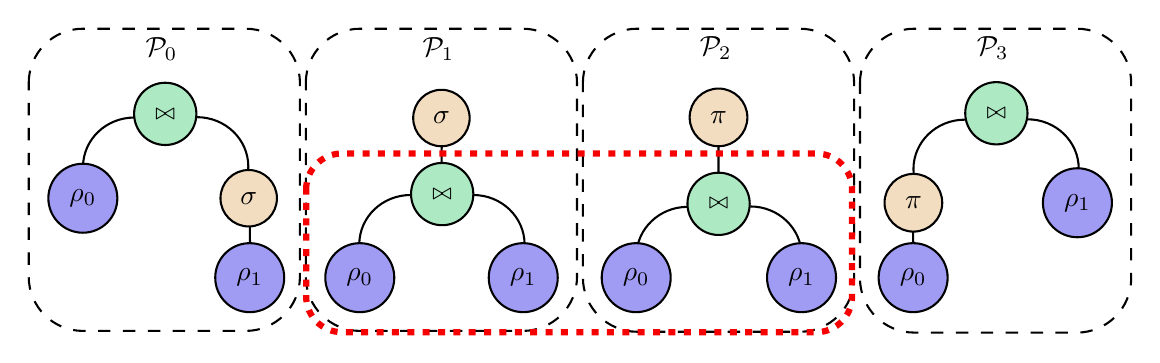
\begin{tikzpicture}[x=0.75pt,y=0.75pt,yscale=-1,xscale=1]
%uncomment if require: \path (0,517); %set diagram left start at 0, and has height of 517

%Rounded Rect [id:dp22693622189021267] 
\draw  [dash pattern={on 4.5pt off 4.5pt}] (105.33,90.93) .. controls (105.33,76.5) and (117.03,64.8) .. (131.47,64.8) -- (209.87,64.8) .. controls (224.3,64.8) and (236,76.5) .. (236,90.93) -- (236,184.27) .. controls (236,198.7) and (224.3,210.4) .. (209.87,210.4) -- (131.47,210.4) .. controls (117.03,210.4) and (105.33,198.7) .. (105.33,184.27) -- cycle ;
%Shape: Arc [id:dp9541025627566715] 
\draw  [draw opacity=0] (131.49,131.2) .. controls (131.6,118.14) and (142.63,107.59) .. (156.22,107.59) -- (156.22,131.41) -- cycle ; \draw   (131.49,131.2) .. controls (131.6,118.14) and (142.63,107.59) .. (156.22,107.59) ;  
%Shape: Arc [id:dp281513038224523] 
\draw  [draw opacity=0] (186.4,107.41) .. controls (200.06,107.41) and (211.13,118.07) .. (211.13,131.22) .. controls (211.13,132.92) and (210.94,134.58) .. (210.59,136.17) -- (186.4,131.22) -- cycle ; \draw   (186.4,107.41) .. controls (200.06,107.41) and (211.13,118.07) .. (211.13,131.22) .. controls (211.13,132.92) and (210.94,134.58) .. (210.59,136.17) ;  
%Straight Lines [id:da9126122398038725] 
\draw    (211.93,172.52) -- (211.92,159.12) ;
%Rounded Rect [id:dp19864875982463825] 
\draw  [dash pattern={on 4.5pt off 4.5pt}] (238.83,90.93) .. controls (238.83,76.5) and (250.53,64.8) .. (264.97,64.8) -- (343.37,64.8) .. controls (357.8,64.8) and (369.5,76.5) .. (369.5,90.93) -- (369.5,184.27) .. controls (369.5,198.7) and (357.8,210.4) .. (343.37,210.4) -- (264.97,210.4) .. controls (250.53,210.4) and (238.83,198.7) .. (238.83,184.27) -- cycle ;
%Shape: Arc [id:dp623273643179123] 
\draw  [draw opacity=0] (264.59,168.54) .. controls (264.7,155.48) and (275.73,144.92) .. (289.32,144.92) -- (289.32,168.74) -- cycle ; \draw   (264.59,168.54) .. controls (264.7,155.48) and (275.73,144.92) .. (289.32,144.92) ;  
%Shape: Arc [id:dp7769680524712608] 
\draw  [draw opacity=0] (319.5,144.92) .. controls (333.16,144.92) and (344.23,155.58) .. (344.23,168.74) -- (319.5,168.74) -- cycle ; \draw   (319.5,144.92) .. controls (333.16,144.92) and (344.23,155.58) .. (344.23,168.74) ;  
%Straight Lines [id:da8996795114234546] 
\draw    (304.18,135.28) -- (304.33,120.33) ;
%Rounded Rect [id:dp7958670756995907] 
\draw  [dash pattern={on 4.5pt off 4.5pt}] (372.33,90.93) .. controls (372.33,76.5) and (384.03,64.8) .. (398.47,64.8) -- (476.87,64.8) .. controls (491.3,64.8) and (503,76.5) .. (503,90.93) -- (503,184.67) .. controls (503,199.1) and (491.3,210.8) .. (476.87,210.8) -- (398.47,210.8) .. controls (384.03,210.8) and (372.33,199.1) .. (372.33,184.67) -- cycle ;
%Shape: Arc [id:dp2653269087913137] 
\draw  [draw opacity=0] (398.09,174.24) .. controls (398.2,161.18) and (409.23,150.62) .. (422.82,150.62) -- (422.82,174.44) -- cycle ; \draw   (398.09,174.24) .. controls (398.2,161.18) and (409.23,150.62) .. (422.82,150.62) ;  
%Shape: Arc [id:dp4205447304867884] 
\draw  [draw opacity=0] (453,150.44) .. controls (453,150.44) and (453,150.44) .. (453,150.44) .. controls (466.66,150.44) and (477.73,161.1) .. (477.73,174.26) -- (453,174.26) -- cycle ; \draw   (453,150.44) .. controls (453,150.44) and (453,150.44) .. (453,150.44) .. controls (466.66,150.44) and (477.73,161.1) .. (477.73,174.26) ;  
%Straight Lines [id:da9337925646863472] 
\draw    (437.68,134.98) -- (437.67,121.58) ;
%Rounded Rect [id:dp8024574861780045] 
\draw  [dash pattern={on 4.5pt off 4.5pt}] (505.83,90.93) .. controls (505.83,76.5) and (517.53,64.8) .. (531.97,64.8) -- (610.37,64.8) .. controls (624.8,64.8) and (636.5,76.5) .. (636.5,90.93) -- (636.5,185.07) .. controls (636.5,199.5) and (624.8,211.2) .. (610.37,211.2) -- (531.97,211.2) .. controls (517.53,211.2) and (505.83,199.5) .. (505.83,185.07) -- cycle ;
%Shape: Arc [id:dp2988707343502508] 
\draw  [draw opacity=0] (532.25,137.94) .. controls (531.82,136.18) and (531.59,134.33) .. (531.59,132.44) .. controls (531.59,119.28) and (542.66,108.62) .. (556.32,108.62) -- (556.32,132.44) -- cycle ; \draw   (532.25,137.94) .. controls (531.82,136.18) and (531.59,134.33) .. (531.59,132.44) .. controls (531.59,119.28) and (542.66,108.62) .. (556.32,108.62) ;  
%Shape: Arc [id:dp10478086547979326] 
\draw  [draw opacity=0] (586.5,108.44) .. controls (586.5,108.44) and (586.5,108.44) .. (586.5,108.44) .. controls (600.16,108.44) and (611.23,119.1) .. (611.23,132.26) .. controls (611.23,132.73) and (611.21,133.2) .. (611.19,133.66) -- (586.5,132.26) -- cycle ; \draw   (586.5,108.44) .. controls (586.5,108.44) and (586.5,108.44) .. (586.5,108.44) .. controls (600.16,108.44) and (611.23,119.1) .. (611.23,132.26) .. controls (611.23,132.73) and (611.21,133.2) .. (611.19,133.66) ;  
%Straight Lines [id:da5382439939318251] 
\draw    (531.48,173.38) -- (531.47,159.98) ;

%Rounded Rect [id:dp22736885699089981] 
\draw  [color={rgb, 255:red, 246; green, 1; blue, 1 }  ,draw opacity=1 ][dash pattern={on 2.53pt off 3.02pt}][line width=2.25]  (239,142.14) .. controls (239,132.63) and (246.71,124.92) .. (256.22,124.92) -- (484.78,124.92) .. controls (494.29,124.92) and (502,132.63) .. (502,142.14) -- (502,193.78) .. controls (502,203.29) and (494.29,211) .. (484.78,211) -- (256.22,211) .. controls (246.71,211) and (239,203.29) .. (239,193.78) -- cycle ;

% Text Node
\draw (427.17,67.23) node [anchor=north west][inner sep=0.75pt]    {$\mathcal{P}_{2}$};
% Text Node
\draw  [fill={rgb, 255:red, 242; green, 221; blue, 192 }  ,fill opacity=1 ]  (437.67, 107.53) circle [x radius= 13.9, y radius= 13.9]   ;
\draw (437.67,107.53) node    {$\pi $};
% Text Node
\draw (560.67,67.23) node [anchor=north west][inner sep=0.75pt]    {$\mathcal{P}_{3}$};
% Text Node
\draw  [fill={rgb, 255:red, 242; green, 221; blue, 192 }  ,fill opacity=1 ]  (531.57, 148.65) circle [x radius= 13.9, y radius= 13.9]   ;
\draw (531.57,148.65) node    {$\pi $};
% Text Node
\draw  [fill={rgb, 255:red, 173; green, 234; blue, 195 }  ,fill opacity=1 ]  (437.71, 149.17) circle [x radius= 15, y radius= 15]   ;
\draw (437.71,149.17) node  [font=\footnotesize]  {$\bowtie $};
% Text Node
\draw  [fill={rgb, 255:red, 173; green, 234; blue, 195 }  ,fill opacity=1 ]  (571.54, 105.53) circle [x radius= 15, y radius= 15]   ;
\draw (571.54,105.53) node  [font=\footnotesize]  {$\bowtie $};
% Text Node
\draw  [fill={rgb, 255:red, 160; green, 156; blue, 243 }  ,fill opacity=1 ]  (398.01, 184.74) circle [x radius= 16.62, y radius= 16.62]   ;
\draw (398.01,184.74) node   [align=left] {$\displaystyle \rho _{0}$};
% Text Node
\draw  [fill={rgb, 255:red, 160; green, 156; blue, 243 }  ,fill opacity=1 ]  (477.67, 184.74) circle [x radius= 16.62, y radius= 16.62]   ;
\draw (477.67,184.74) node   [align=left] {$\displaystyle \rho _{1}$};
% Text Node
\draw  [fill={rgb, 255:red, 160; green, 156; blue, 243 }  ,fill opacity=1 ]  (531.44, 184.74) circle [x radius= 16.62, y radius= 16.62]   ;
\draw (531.44,184.74) node   [align=left] {$\displaystyle \rho _{0}$};
% Text Node
\draw  [fill={rgb, 255:red, 160; green, 156; blue, 243 }  ,fill opacity=1 ]  (610.59, 148.65) circle [x radius= 16.62, y radius= 16.62]   ;
\draw (610.59,148.65) node   [align=left] {$\displaystyle \rho _{1}$};
% Text Node
\draw (160.17,67.53) node [anchor=north west][inner sep=0.75pt]    {$\mathcal{P}_{0}$};
% Text Node
\draw (293.67,67.53) node [anchor=north west][inner sep=0.75pt]    {$\mathcal{P}_{1}$};
% Text Node
\draw  [fill={rgb, 255:red, 242; green, 221; blue, 192 }  ,fill opacity=1 ]  (304.17, 107.83) circle [x radius= 13.6, y radius= 13.6]   ;
\draw (304.17,107.83) node    {$\sigma $};
% Text Node
\draw  [fill={rgb, 255:red, 173; green, 234; blue, 195 }  ,fill opacity=1 ]  (304.54, 144.47) circle [x radius= 15, y radius= 15]   ;
\draw (304.54,144.47) node  [font=\footnotesize]  {$\bowtie $};
% Text Node
\draw  [fill={rgb, 255:red, 160; green, 156; blue, 243 }  ,fill opacity=1 ]  (264.84, 184.74) circle [x radius= 16.62, y radius= 16.62]   ;
\draw (264.84,184.74) node   [align=left] {$\displaystyle \rho _{0}$};
% Text Node
\draw  [fill={rgb, 255:red, 160; green, 156; blue, 243 }  ,fill opacity=1 ]  (343.59, 184.74) circle [x radius= 16.62, y radius= 16.62]   ;
\draw (343.59,184.74) node   [align=left] {$\displaystyle \rho _{1}$};
% Text Node
\draw  [fill={rgb, 255:red, 173; green, 234; blue, 195 }  ,fill opacity=1 ]  (171.11, 105.83) circle [x radius= 15, y radius= 15]   ;
\draw (171.11,105.83) node  [font=\footnotesize]  {$\bowtie $};
% Text Node
\draw  [fill={rgb, 255:red, 160; green, 156; blue, 243 }  ,fill opacity=1 ]  (131.41, 146.47) circle [x radius= 16.62, y radius= 16.62]   ;
\draw (131.41,146.47) node   [align=left] {$\displaystyle \rho _{0}$};
% Text Node
\draw  [fill={rgb, 255:red, 160; green, 156; blue, 243 }  ,fill opacity=1 ]  (211.81, 184.74) circle [x radius= 16.62, y radius= 16.62]   ;
\draw (211.81,184.74) node   [align=left] {$\displaystyle \rho _{1}$};
% Text Node
\draw  [fill={rgb, 255:red, 242; green, 221; blue, 192 }  ,fill opacity=1 ]  (211.32, 146.47) circle [x radius= 13.6, y radius= 13.6]   ;
\draw (211.32,146.47) node    {$\sigma $};


\end{tikzpicture}


    \caption{4 different query plans $\mathcal{P}_0$, $\mathcal{P}_1$ for query $\mathcal{Q}_0$ and $\mathcal{P}_2$, $\mathcal{P}_3$ for query $\mathcal{Q}_1$. The plans have different ordered instructions, which can save time during single execution or allow for more parallel savings.}
    \label{figure:4_query_plans}
\end{figure}

The plans from figure \ref{figure:4_query_plans} are built to best resemble the costs and savings defined in the data from listing \ref{figure:2d_problem_data}. As per said listing, the combination of $\mathcal{P}_1$ and $\mathcal{P}_2$ offers the greatest savings. In this case, the step that would warrant such savings would be $\rho_0\bowtie\rho_1$, that is present in both plans, and surrounded with a red rectangle. In every other case, there are preliminary operations that change the result so that it is not shareable by the plans. Nevertheless, one could still share single steps like $\rho_0$ and $\rho_1$.

\newpage

The problem space from listing \ref{figure:2d_problem_data} is used for direct comparison between our solution and the solution of Fankhauer et al.\cite{fankhauser_multiple_2021}. As one cannot assume that real life problems will always be limited to 2 queries with 2 problems each, the problem generator is enhanced to allow for any number of queries, each of which with their own number of plans, as shown in figure \ref{figure:nd_problem_data}.

\begin{listing}[!ht]
    \centering
    \begin{minted}{python}
        ([2, 3, 2],
          [21,  1, 36, 16, 33, 42,  7],
          {(0, 2): -7,
           (0, 3): -13,
           (0, 4): -14,
           (0, 5): -6,
           (0, 6): 0,
           (1, 2): -18,
           (1, 3): -12,
           (1, 4): -17,
           (1, 5): -14,
           (1, 6): -4,
           (2, 5): -5,
           (2, 6): -6,
           (3, 5): -20,
           (3, 6): -12,
           (4, 5): -10,
           (4, 6): 0})
    \end{minted}
    \caption{This is an automatically generated, $n$-dimensional problem space $\mathcal{D}$. The first array tells us how many plans each query has. This problem has 3 queries, two of which have 2 plans and one with 3 plans. Just like the problem from listing \ref{figure:2d_problem_data}, the second element is an array that contains the cost of each plan, and the third element, which is a dictionary, contains the combinations keys and their respective savings.}
    \label{figure:nd_problem_data}
\end{listing}

\newpage

\subsection{Circuit Design}
\label{chapter:circuit_design}

The design of the circuit is carefully modelled as to allow easier understanding of its behaviour. As a baseline for the choice of gates, the work of Sim et al.\cite{sim_expressibility_2019} states that using differing Pauli-Gates increases the traversable state space, which therefore allows the circuit to deliver better results. This is used to decide on which gates to use. At the same time, we follow the statements from chapter \ref{chapter:qnn}. \par
Initially, for any $n$ plans, the probabilities of each being the cheapest is unknown, which directly means they are all \emph{equally probable}. To realize this, the circuit has one qubit per avaliable plan. To create equal probabilities for all plans, an initial layer consisting of one \hgate\ per qubit is constructed, as illustrated in figure \ref{figure:4_qubit_circuit_with_h_gates}.

\begin{figure}[!h]
    \centering
    \scalebox{1.0}{
    \Qcircuit @C=1.0em @R=0.2em @!R { \\
	 	\nghost{{\mathcal{P}}_{0} :  } & \lstick{{\mathcal{P}}_{0} :  } \barrier[0em]{3} & \qw & \gate{\mathrm{H}} \barrier[0em]{3} & \qw & \qw & \qw\\
	 	\nghost{{\mathcal{P}}_{1} :  } & \lstick{{\mathcal{P}}_{1} :  } & \qw & \gate{\mathrm{H}} & \qw & \qw & \qw\\
	 	\nghost{{\mathcal{P}}_{2} :  } & \lstick{{\mathcal{P}}_{2} :  } & \qw & \gate{\mathrm{H}} & \qw & \qw & \qw\\
	 	\nghost{{\mathcal{P}}_{3} :  } & \lstick{{\mathcal{P}}_{3} :  } & \qw & \gate{\mathrm{H}} & \qw & \qw & \qw\\
	 	\nghost{} & \lstick{} & \ket{\psi_0} &  & \ket{\psi_1}\\
\\ }}
    \caption{A 4 qubit circuit (here the qubits are not denoted with $q_i$ but $\mathcal{P}_i$, which represent for each plan in the problem) for the problem defined in figure \ref{figure:2d_problem_data} consisting of only \hgate s to create an equal superposition across all plans}
    \label{figure:4_qubit_circuit_with_h_gates}
\end{figure}

\begin{equation}
    \centering
    \begin{split}
        \mathcal{P}_i =\ \ket{0} &=\ \ket{\psi_0} =\ \begin{pmatrix}1 \\ 0\end{pmatrix}\\
        \mathrm{H}\mathcal{P}_i =\ \mathrm{H}\ket{0} &=\ \frac{1}{\sqrt{2}}\ket{0} + \frac{1}{\sqrt{2}}\ket{1} =\ \begin{pmatrix}\frac{1}{\sqrt{2}} \\ \frac{1}{\sqrt{2}}\end{pmatrix} =\ \ket{\psi_1}\\
        |\bra{1}\ket{\psi_1}_{\mathrm{P}_0}|^2 &=\ \left|\frac{1}{\sqrt{2}}\right|^2 =\ 0.5\\
        |\bra{0}\ket{\psi_1}_{\mathrm{P}_0}|^2 &=\ \left|\frac{1}{\sqrt{2}}\right|^2 =\ 0.5\\
    \end{split}
    \label{equation:2d_problem_state_0_1}
\end{equation}

Whereas at position $\ket{\psi_0}$ all qubits have the state $\ket{0}$, after applying the \hgate s, all the qubits have the state $\frac{1}{\sqrt{2}}\ket{0} + \frac{1}{\sqrt{2}}\ket{1}$ at position $\ket{\psi_1}$.

\subsection{Cost Embedding}
\label{chapter:cost_embedding}

The idea behind the design of the cost embedding onto the quantum circuit is relatively simple. The more expensive a single plan $\mathcal{P}_i$ is, the less its probability to be $1$ should be. To do this, a \rygate\ gate is used per qubit, which can change the probabilities towards $\ket{0}$ or $\ket{1}$. In the end, the probability for $\ket{1}$ should \emph{decrease} with a high cost in the problem space, and \emph{increase} with a low cost. This is analogous to the feature encoding referenced in chapter \ref{chapter:qnn}.

\newpage

\begin{figure}[!h]
    \centering
    \scalebox{1.0}{
    \Qcircuit @C=1.0em @R=0.2em @!R { \\
	 	\nghost{{q}_{0} :  } & \lstick{{\mathcal{P}}_{0} :  } & \gate{\mathrm{H}} & \gate{\mathrm{R_Y}\,(\mathrm{c_0})} \barrier[0em]{3} & \qw & \qw & \qw\\
	 	\nghost{{q}_{1} :  } & \lstick{{\mathcal{P}}_{1} :  } & \gate{\mathrm{H}} & \gate{\mathrm{R_Y}\,(\mathrm{c_1})} & \qw & \qw & \qw\\
	 	\nghost{{q}_{2} :  } & \lstick{{\mathcal{P}}_{2} :  } & \gate{\mathrm{H}} & \gate{\mathrm{R_Y}\,(\mathrm{c_2})} & \qw & \qw & \qw\\
	 	\nghost{{q}_{3} :  } & \lstick{{\mathcal{P}}_{3} :  } & \gate{\mathrm{H}} & \gate{\mathrm{R_Y}\,(\mathrm{c_3})} & \qw & \qw & \qw\\
	 	\nghost{} : & \lstick{{} } & & & \ket{\psi_2}& \\
    \\ }}
    \caption{The 4 qubit circuit from figure \ref{figure:4_qubit_circuit_with_h_gates} for the problem defined in listing \ref{figure:2d_problem_data} extended with cost encoding \rygate.}
    \label{figure:4_qubit_circuit_with_h_ry_gates}
\end{figure}

\begin{equation}
    \centering
    \begin{split}
        \mathrm{RY}(c_i)\mathrm{H}\mathcal{P}_i &=\ \begin{pmatrix} \cos{\frac{c_i}{2}} & -\sin{\frac{c_i}{2}} \\ \sin{\frac{c_i}{2}} & \cos{\frac{c_i}{2}} \end{pmatrix}\begin{pmatrix}\frac{1}{\sqrt{2}} \\ \frac{1}{\sqrt{2}}\end{pmatrix}\\
        \mathrm{RY}(c_i)\mathrm{H}\mathcal{P}_i &=\ \frac{1}{\sqrt{2}}\begin{pmatrix}\cos(\frac{c_i}{2}) - \sin(\frac{c_i}{2}) \\ \sin(\frac{c_i}{2}) + \cos(\frac{c_i}{2})\end{pmatrix} =\ \ket{\psi_2}\\
    \end{split}
    \label{equation:2d_problem_state_0_1}
\end{equation}

\begin{equation}
    \centering
    \begin{split}
        c_0 &=\ 0.5\\
        c_1 &=\ -0.5\\
        |\bra{0}\ket{\psi_2}_{\mathrm{P_0}}|^2 &=\ 0.2603 \\
        |\bra{1}\ket{\psi_2}_{\mathrm{P_0}}|^2 &=\ 0.7397 \\
        |\bra{0}\ket{\psi_2}_{\mathrm{P_1}}|^2 &=\ 0.7397 \\
        |\bra{1}\ket{\psi_2}_{\mathrm{P_1}}|^2 &=\ 0.2603 \\
    \end{split}
    \label{equation:2d_problem_state_measurements}
\end{equation}

As equation \ref{equation:2d_problem_state_measurements} shows, the opposite happens. This can be easily corrected by multiplying the cost with a factor of $-1$, with the corrected circuit shown in figure \ref{figure:4_qubit_circuit_with_h_neg_ry_gates}. Before the cost is applied, any qubit in the given circuit from figure \ref{figure:4_qubit_circuit_with_h_ry_gates} has the state shown in figure \ref{figure:q_sphere_no_cost}. Applying the cost factors, a high-cost \emph{increases} the chances of measuring $0$, as shown in figure \ref{figure:q_sphere_bad_cost} whereas a low-cost increases the chances of measuring a $1$, as demonstrate in figure \ref{figure:q_sphere_good_cost}. 


\begin{figure}[!h]
    \centering
    \scalebox{1.0}{
    \Qcircuit @C=1.0em @R=0.2em @!R { \\
	 	\nghost{{q}_{0} :  } & \lstick{{\mathcal{P}}_{0} :  } & \gate{\mathrm{H}} & \gate{\mathrm{R_Y}\,(-\mathrm{c_0})} \barrier[0em]{3} & \qw & \qw & \qw\\
	 	\nghost{{q}_{1} :  } & \lstick{{\mathcal{P}}_{1} :  } & \gate{\mathrm{H}} & \gate{\mathrm{R_Y}\,(-\mathrm{c_1})} & \qw & \qw & \qw\\
	 	\nghost{{q}_{2} :  } & \lstick{{\mathcal{P}}_{2} :  } & \gate{\mathrm{H}} & \gate{\mathrm{R_Y}\,(-\mathrm{c_2})} & \qw & \qw & \qw\\
	 	\nghost{{q}_{3} :  } & \lstick{{\mathcal{P}}_{3} :  } & \gate{\mathrm{H}} & \gate{\mathrm{R_Y}\,(-\mathrm{c_3})} & \qw & \qw & \qw\\
	 	\nghost{} : & \lstick{{} } & & & \ket{\psi_2}& \\
    \\ }}
    \caption{The 4 qubit circuit from figure \ref{figure:4_qubit_circuit_with_h_ry_gates} with negated parameter $c_i$, so that the probabilities move correctly according to the cost of each plan $\mathrm{P}_i$.}
    \label{figure:4_qubit_circuit_with_h_neg_ry_gates}
\end{figure}


\begin{figure}[!h]
    \centering
    \scalebox{\histogramwidth}{
        \includesvg{thesis/Appendices/Q_Sphere_State_h.svg}
    }
    \caption{A Q-Sphere showing the state of a single qubit (representing a plan $\mathcal{P}_i$), where the probabilities of $\ket{0}$ and $\ket{1}$ are equal.}
    \label{figure:q_sphere_no_cost}
\end{figure}

\begin{figure}[!h]
    \centering
    \scalebox{\histogramwidth}{
        \includesvg{thesis/Appendices/Q_Sphere_State_ry_-0_5.svg}
    }
    \caption{A Q-Sphere that shows the state of a single qubit (representing a plan $\mathcal{P}_i$), where the cost $0.5$ was embedded onto state \ref{figure:q_sphere_no_cost} and therefore the probability of a $\ket{0}$ increased.}
    \label{figure:q_sphere_bad_cost}
\end{figure}

\begin{figure}[!h]
    \centering
    \scalebox{\histogramwidth}{
        \includesvg{thesis/Appendices/Q_Sphere_State_ry_0_5.svg}
    }
    \caption{A Q-Sphere that shows the state of a single qubit (representing a plan $\mathcal{P}_i$), where the cost $-0.5$ was embedded onto state \ref{figure:q_sphere_no_cost} and therefore the probability of a $\ket{1}$ increased.}
    \label{figure:q_sphere_good_cost}
\end{figure}

\clearpage

\subsection{Savings Embedding}

As contrary to normal problem spaces our data has combinational features that involve multiple plans, the \crzgate\ is used, which entangles two qubits and adds another dimensionality to the problem space the circuit can traverse. For two plans \plani\ and \planj\ to be entangled, the rule \ref{equation:entanglement_rule} has to be true. If it is, the pair-wise savings are applied.

\begin{equation}
\centering
    \begin{split}
        \forall\  \mathcal{P}_i,\ \mathcal{P}_j,\ \mathcal{Q}_a,\ \mathcal{Q}_b &\in\ \mathcal{D}\ \\ 
        i \neq j \wedge\ a \neq b \wedge\ \left(\mathcal{P}_i\ \in\ \mathcal{Q}_a\ \wedge \mathcal{P}_j\ \notin\ \mathcal{Q}_a\right) &\wedge\ \left(\mathcal{P}_j\ \in\ \mathcal{Q}_b\ \wedge \mathcal{P}_i\ \notin\ \mathcal{Q}_b\right)\\
    \end{split}
    \label{equation:entanglement_rule}
\end{equation}


As defined for a problem space in listing \ref{figure:2d_problem_data}, the savings themselves are negative. A circuit with all data embeddings is visualized in figure \ref{figure:4_qubit_circuit_with_h_ry_crz_gates}.

\begin{figure}[!h]
    \centering
    \scalebox{1.0}{
\Qcircuit @C=1.0em @R=0.2em @!R { \\
	 	\nghost{{q}_{0} :  } & \lstick{{\mathcal{P}}_{0}  :  } & \gate{\mathrm{H}} & \gate{\mathrm{R_Y}\,(\mathrm{-c_0})} & \ctrl{2} & \ctrl{3} & \qw & \qw \barrier[0em]{3} & \qw & \qw & \qw\\
	 	\nghost{{q}_{1} :  } & \lstick{{\mathcal{P}}_{1}  :  } & \gate{\mathrm{H}} & \gate{\mathrm{R_Y}\,(\mathrm{-c_1})} & \qw & \qw & \ctrl{1} & \ctrl{2} & \qw & \qw & \qw\\
	 	\nghost{{q}_{2} :  } & \lstick{{\mathcal{P}}_{2}  :  } & \gate{\mathrm{H}} & \gate{\mathrm{R_Y}\,(\mathrm{-c_2})} & \gate{\mathrm{R_Z}\,(\mathrm{s_{02}})} & \qw & \gate{\mathrm{R_Z}\,(\mathrm{s_{12}})} & \qw & \qw & \qw & \qw\\
	 	\nghost{{q}_{3} :  } & \lstick{{\mathcal{P}}_{3}  :  } & \gate{\mathrm{H}} & \gate{\mathrm{R_Y}\,(\mathrm{-c_3})} & \qw & \gate{\mathrm{R_Z}\,(\mathrm{s_{03}})} & \qw & \gate{\mathrm{R_Z}\,(\mathrm{s_{13}})} & \qw & \qw & \qw\\
	 	\nghost{ } & \lstick{ } & & & & & & & \ket{\psi_3} & &\\
\\ }}
    \caption{A 4 qubit circuit with an equal probability layer, the cost embedding layer from \ref{figure:4_qubit_circuit_with_h_ry_gates} as well as a new \crzgate\ layer to embed the combinational savings of single pairs of plans.}
    \label{figure:4_qubit_circuit_with_h_ry_crz_gates}
\end{figure}

\subsection{Data}

The goal of this research is to evaluate a circuit, that in the future can be used to greatly speed up query combination on real database systems. This demands strict forethought about the way the data is handled. One problem that exists is that the cost values are, by themselves, not limited to a given range. This means that whilst the generated data might have a limited range, one cannot reassure that any real life data will stay within that range. This leads to the choice of normalizing \emph{each problem by itself}, instead of the usual approach in machine learning of normalizing a complete datasets. This allows to somewhat bring structure into the problem space $\mathcal{D}$. Equations \ref{equation:normalization_range_1} to \ref{equation:normalization_range_forth_pi} use the \rygate\ with different parameters to show the result the value has on the probabilities of $\ket{0}$ and $\ket{1}$.

\begin{equation}
    \centering
    \begin{split}
        \mathrm{RY}(1)\mathrm{H}\ket{0} &=\ \frac{1}{\sqrt{2}}\begin{pmatrix}\cos(\frac{1}{2}) \\ \sin(\frac{1}{2})\end{pmatrix}\\
        \ket{0} &\to 0.079 \\
        \ket{1} &\to 0.921 \\
        \mathrm{RY}(-1)\mathrm{H}\ket{0} &=\ \frac{1}{\sqrt{2}}\begin{pmatrix}\cos(\frac{-1}{2}) \\ \sin(\frac{-1}{2})\end{pmatrix}\\
        \ket{0} &\to 0.918 \\
        \ket{1} &\to 0.082 \\
    \end{split}
    \label{equation:normalization_range_1}
\end{equation}

\begin{equation}
    \centering
    \begin{split}
        \mathrm{RY}(1.5)\mathrm{H}\ket{0} &=\ \frac{1}{\sqrt{2}}\begin{pmatrix}\cos(\frac{1.5}{2}) \\ \sin(\frac{1.5}{2})\end{pmatrix}\\
        \ket{0} &\to 0.002 \\
        \ket{1} &\to 0.998 \\
        \mathrm{RY}(-1.5)\mathrm{H}\ket{0} &=\ \frac{1}{\sqrt{2}}\begin{pmatrix}\cos(\frac{-1.5}{2}) \\ \sin(\frac{-1.5}{2})\end{pmatrix}\\
        \ket{0} &\to 0.999 \\
        \ket{1} &\to 0.001 \\
    \end{split}
    \label{equation:normalization_range_1_5}
\end{equation}

\begin{equation}
    \centering
    \begin{split}
        \mathrm{RY}(2)\mathrm{H}\ket{0} &=\ \frac{1}{\sqrt{2}}\begin{pmatrix}\cos(\frac{2}{2}) \\ \sin(\frac{2}{2})\end{pmatrix}\\
        \ket{0} &\to 0.047 \\
        \ket{1} &\to 0.953 \\
        \mathrm{RY}(-2)\mathrm{H}\ket{0} &=\ \frac{1}{\sqrt{2}}\begin{pmatrix}\cos(\frac{-2}{2}) \\ \sin(\frac{-2}{2})\end{pmatrix}\\
        \ket{0} &\to 0.948 \\
        \ket{1} &\to 0.052 \\
    \end{split}
    \label{equation:normalization_range_2}
\end{equation}

\begin{equation}
    \centering
    \begin{split}
        \mathrm{RY}(\pi)\mathrm{H}\ket{0} &=\ \frac{1}{\sqrt{2}}\begin{pmatrix}\cos(\frac{\pi}{2}) \\ \sin(\frac{\pi}{2})\end{pmatrix}\\
        \ket{0} &\to 0.495 \\
        \ket{1} &\to 0.505 \\
        \mathrm{RY}(-\pi)\mathrm{H}\ket{0} &=\ \frac{1}{\sqrt{2}}\begin{pmatrix}\cos(\frac{-\pi}{2}) \\ \sin(\frac{-\pi}{2})\end{pmatrix}\\
        \ket{0} &\to 0 \\
        \ket{1} &\to 1 \\
    \end{split}
    \label{equation:normalization_range_pi}
\end{equation}

\begin{equation}
    \centering
    \begin{split}
        \mathrm{RY}(\frac{\pi}{2})\mathrm{H}\ket{0} &=\ \frac{1}{\sqrt{2}}\begin{pmatrix}\cos(\frac{\pi}{4}) \\ \sin(\frac{\pi}{4})\end{pmatrix}\\
        \ket{0} &\to 0 \\
        \ket{1} &\to 1 \\
        \mathrm{RY}(-\frac{\pi}{2})\mathrm{H}\ket{0} &=\ \frac{1}{\sqrt{2}}\begin{pmatrix}\cos(\frac{-\pi}{4}) \\ \sin(\frac{-\pi}{4})\end{pmatrix}\\
        \ket{0} &\to 1 \\
        \ket{1} &\to 0 \\
    \end{split}
    \label{equation:normalization_range_half_pi}
\end{equation}

\begin{equation}
    \centering
    \begin{split}
        \mathrm{RY}(\frac{\pi}{4})\mathrm{H}\ket{0} &=\ \frac{1}{\sqrt{2}}\begin{pmatrix}\cos(\frac{\pi}{8}) \\ \sin(\frac{\pi}{8})\end{pmatrix}\\
        \ket{0} &\to 0.142 \\
        \ket{1} &\to 0.858 \\
        \mathrm{RY}(-\frac{\pi}{4})\mathrm{H}\ket{0} &=\ \frac{1}{\sqrt{2}}\begin{pmatrix}\cos(\frac{-\pi}{8}) \\ \sin(\frac{-\pi}{8})\end{pmatrix}\\
        \ket{0} &\to 0.862 \\
        \ket{1} &\to 0.138 \\
    \end{split}
    \label{equation:normalization_range_forth_pi}
\end{equation}

As defined in chapter \ref{chapter:circuit_design}, the qubits are in an equal superposition before the \rygate\ is applied. Chapter \ref{chapter:cost_embedding} also defines that the probability has to be able to increase for either $\ket{0}$ or $\ket{1}$. Equations \ref{equation:normalization_range_1}, \ref{equation:normalization_range_1_5} and \ref{equation:normalization_range_2} show an overflow when manipulating probabilities. They imply that there is a tipping point between $2$ and $1$, when coming from an equal superposition, where the probabilities start decreasing again. As gates like \rygate\ use $\cos$ and $\sin$, equation \ref{equation:normalization_range_pi} uses $\pi$ to analyse the behaviour. The results dictate that the manipulation with $\pi$ leaves the probabilities to what they are when only applying $\mathrm{H}\ket{0}$. \par
The exact value to set the probability of one state to $1$ ends up being $\frac{\pi}{2}$, as equation \ref{equation:normalization_range_half_pi} shows. Depending on problem space $\mathcal{D}$, the number of parameters being embedded into a qubit can be higher or lower. As going over the supposed \emph{tipping point} of probabilities would mean a loss of information, a lower range is needed. Equation \ref{equation:normalization_range_half_pi} shows this in action, which delivers acceptable state probabilities.\par
The code from listing \ref{code:normalization_code} handles normalizing all problem data, using scikits\cite{scikit-learn} \code{MinMaxScaler}, generated from the function described in chapter \ref{chapter:mqo_data_acquisition}. It is important to note that the normalization is done \emph{per problem}, and not for the whole dataset. This means that the highest cost per problem will always be $\frac{\pi}{4}$, and the greatest savings $-\frac{\pi}{4}$.

\clearpage

\begin{listing}[!h]
    \centering
    \begin{minted}{python}
        import numpy as np
        from sklearn.preprocessing import MinMaxScaler
        
        scaler = MinMaxScaler((-np.pi/4, np.pi/4))
        scaled_problems = []
        for problem in problems:
            scaled_problems.append(scaler.fit_transform(
                            problem.reshape(-1,1)))
    \end{minted}
    \caption{Python code to normalize all values of a problem space $\mathcal{D}$ to the range $\left[-\frac{\pi}{4},\frac{\pi}{4}\right]$}
    \label{code:normalization_code}
\end{listing}

After scaling the data, it is applied directly onto the corresponding gates of a circuit. For the problem space $\mathcal{D}$ illustrated in listing \ref{figure:2d_problem_data} and shown in normalized form in listing \ref{listing:2d_problem_data_normalized}, the circuit \ref{circuit:example_mqo_solver_circuit_for_2d_problem_data} can be used to solve the problem.

\begin{listing}[!ht]
    \centering
    \begin{minted}{python}
        [ 0.15707963, 0.78539816, 0.20943951, -0.15707963,
         -0.60213859, -0.54977871, -0.78539816, -0.60213859]
    \end{minted}
    \caption{The problem data from figure \ref{figure:2d_problem_data} in normalized form after being passed through the normalizer from figure \ref{code:normalization_code}. The first row resembles the costs of plans $\mathcal{P}_0$ to $\mathcal{P}_3$, and the second row resembles the possible savings for combinations $\mathcal{P}_0\mathcal{P}_2$, $\mathcal{P}_0\mathcal{P}_3$, $\mathcal{P}_1\mathcal{P}_2$ and $\mathcal{P}_1\mathcal{P}_3$.}
    \label{listing:2d_problem_data_normalized}
\end{listing}

\begin{figure}[!h]
    \centering
    \scalebox{0.8}{
\Qcircuit @C=1.0em @R=0.2em @!R { \\
	 	\nghost{{q}_{0} :  } & \lstick{{q}_{0} :  } & \gate{\mathrm{H}} & \gate{\mathrm{R_Y}\,(\frac{-\pi}{20})} & \ctrl{2} & \ctrl{3} & \qw & \qw & \qw & \qw\\
	 	\nghost{{q}_{1} :  } & \lstick{{q}_{1} :  } & \gate{\mathrm{H}} & \gate{\mathrm{R_Y}\,(\frac{-\pi}{4})} & \qw & \qw & \ctrl{1} & \ctrl{2} & \qw & \qw\\
	 	\nghost{{q}_{2} :  } & \lstick{{q}_{2} :  } & \gate{\mathrm{H}} & \gate{\mathrm{R_Y}\,(\frac{-\pi}{15})} & \gate{\mathrm{R_Z}\,(\mathrm{-0.6021})} & \qw & \gate{\mathrm{R_Z}\,(\frac{-\pi}{4})} & \qw & \qw & \qw\\
	 	\nghost{{q}_{3} :  } & \lstick{{q}_{3} :  } & \gate{\mathrm{H}} & \gate{\mathrm{R_Y}\,(\frac{\pi}{20})} & \qw & \gate{\mathrm{R_Z}\,(\mathrm{-0.5498})} & \qw & \gate{\mathrm{R_Z}\,(\mathrm{-0.6021})} & \qw & \qw\\
\\ }}
    \caption{The circuit with all normalized parameters from listing \ref{listing:2d_problem_data_normalized} embedded onto it.}
    \label{circuit:example_mqo_solver_circuit_for_2d_problem_data}
\end{figure}

To allow for direct comparison of alternative solutions, a general dataset $\mathcal{D}_{2\times2}$ is generated, and divided into a \emph{training} subset $\mathcal{D}_{train} \subset \mathcal{D}_{2\times2}$ and a \emph{training} subset $\mathcal{D}_{test} \subset \mathcal{D}_{2\times2}$, where the spread is 0.75 for training, and 0.25 for testing. The total size being $\left|\mathcal{D}_{2\times2}\right| =\ 300$.


\subsection{Machine Learning}
\label{chapter:mqo_machine_learning}

To enable an optimizer to train the circuit defined in chapter \ref{chapter:circuit_design}, parameters have to be created which can be set as to best solve the given task. In chapter \ref{chapter:qnn}, this is referred to as the variational circuit that is optimized. As stated in chapter \ref{chapter:circuit_design}, a mixture of different gates allows the traversal of a wider space, which helps in finding suitable solutions. As the circuit already uses \rygate s and \crzgate s, which cover the Pauli matrices $\mathrm{Y}$ and $\mathrm{Z}$, the gates that will be parameterized with trainable weight are \rxgate s. Each qubit receives its own, non entangled \rxgate\ with its trainable parameter $\theta_i$, as shown in figure \ref{circuit:full_trainable_mqp_circuit}.

\begin{figure}[!h]
    \centering
    \scalebox{0.8}{
\Qcircuit @C=1.0em @R=0.2em @!R { \\
	 	\nghost{{q}_{0} :  } & \lstick{{q}_{0} :  } & \gate{\mathrm{H}} & \gate{\mathrm{R_Y}\,(\mathrm{c_0})} & \ctrl{2} & \ctrl{3}  & \qw & \qw & \gate{\mathrm{R_X}\,(\theta_0)} & \qw & \qw\\
	 	\nghost{{q}_{1} :  } & \lstick{{q}_{1} :  } & \gate{\mathrm{H}} & \gate{\mathrm{R_Y}\,(\mathrm{c_1})} & \qw & \qw & \ctrl{1} & \ctrl{2} & \gate{\mathrm{R_X}\,(\theta_1)} & \qw & \qw\\
	 	\nghost{{q}_{2} :  } & \lstick{{q}_{2} :  } & \gate{\mathrm{H}} & \gate{\mathrm{R_Y}\,(\mathrm{c_2})} & \gate{\mathrm{R_Z}\,(\mathrm{s_{02}})} & \qw & \gate{\mathrm{R_Z}\,(\mathrm{s_{12}})} & \qw & \gate{\mathrm{R_X}\,(\theta_2)} & \qw & \qw\\
	 	\nghost{{q}_{3} :  } & \lstick{{q}_{3} :  } & \gate{\mathrm{H}} & \gate{\mathrm{R_Y}\,(\mathrm{c_3})} & \qw & \gate{\mathrm{R_Z}\,(\mathrm{s_{03}})} & \qw & \gate{\mathrm{R_Z}\,(\mathrm{s_{13}})} & \gate{\mathrm{R_X}\,(\theta_3)} & \qw & \qw\\
\\ }}
    \caption{The full MQO solver circuit for a problem space $\mathcal{D}_{2\times2}$ with one full layer of \rxgate s with trainable weights $\theta_i$ as parameters.}
    \label{circuit:full_trainable_mqp_circuit}
\end{figure}

\subsubsection{Manual Validation}
\label{chapter:mqo_manual_validation}
To assess that the circuit from figure \ref{circuit:full_trainable_mqp_circuit} is able to correctly handle the generated problem as well as deliver usable results, a static variant is created where the \rxgate\ has a static value. As previously shown, $\frac{\pi}{4}$ appears to be a good value for normalization, so this is also used in the static variant as the variable for the \rxgate\ layer, as shown in figure \ref{circuit:static_mqo_circuit}.\par
As each avaliable plan is represented by one qubit, and previous chapters designed the circuit in a fashion so that cheap plans are more inclined to be measured as $1$, there are four possible keys: $\{1010, 1001, 0110, 0101\}$ in the problem space $\mathcal{D}_{2\times2}$. With this information in mind, the measurements taken are filtered before evaluation. This means that any state $S \notin \{1010, 1001, 0110, 0101\}$ is removed. Afterwards, the state with the highest probability is taken.

\begin{figure}[!h]
    \centering
    \scalebox{0.8}{
\Qcircuit @C=1.0em @R=0.2em @!R { \\
	 	\nghost{{q}_{0} :  } & \lstick{{q}_{0} :  } & \gate{\mathrm{H}} & \gate{\mathrm{R_Y}\,(\mathrm{c_0})} & \ctrl{2} & \ctrl{3} & \qw & \qw & \gate{\mathrm{R_X}\,(\frac{\pi}{4})} & \qw & \qw \\
	 	\nghost{{q}_{1} :  } & \lstick{{q}_{1} :  } & \gate{\mathrm{H}} & \gate{\mathrm{R_Y}\,(\mathrm{c_1})} & \qw & \qw & \ctrl{1} & \ctrl{2} & \gate{\mathrm{R_X}\,(\frac{\pi}{4})} & \qw & \qw\\
	 	\nghost{{q}_{2} :  } & \lstick{{q}_{2} :  } & \gate{\mathrm{H}} & \gate{\mathrm{R_Y}\,(\mathrm{c_2})} & \gate{\mathrm{R_Z}\,(\mathrm{s_02})} & \qw & \gate{\mathrm{R_Z}\,(\mathrm{s_12})} & \qw & \gate{\mathrm{R_X}\,(\frac{\pi}{4})} & \qw & \qw\\
	 	\nghost{{q}_{3} :  } & \lstick{{q}_{3} :  } & \gate{\mathrm{H}} & \gate{\mathrm{R_Y}\,(\mathrm{c_3})} & \qw & \gate{\mathrm{R_Z}\,(\mathrm{s_03})} & \qw & \gate{\mathrm{R_Z}\,(\mathrm{s_13})} & \gate{\mathrm{R_X}\,(\frac{\pi}{4})} & \qw & \qw\\
\\ }}
    \caption{A static variant of the circuit \ref{circuit:full_trainable_mqp_circuit} where the \rxgate\ layer was fitted with the static value $\frac{\pi}{4}$, to allow for manual execution, evaluation and as assessment for the viability of the circuit.}
    \label{circuit:static_mqo_circuit}
\end{figure}

The circuit \ref{circuit:static_mqo_circuit} is run with a randomly generated problem space $\left|\mathcal{D}_{2\times2}\right| =\ 5000$. This size was chosen to allow any specific edge cases to appear and be handled. In addition, each measurement is taken with 1024 shots, a standard value used in the library \code{qiskit}. The experiment runs 13 times and the results are summarized in figure \ref{figure:boxplot_static_circuit_accuracies}.

\newpage

\begin{figure}[!ht]
    \centering
    \scalebox{0.6}{
        \includesvg{thesis/Appendices/static_circuit_accuracies_boxplot.svg}
    }
    \caption{Achieved accuracies after 13 runs on the generated problem space $\left|\mathcal{D}_{2\times2}\right| =\ 5000$ with 1024 shots each, using the circuit \ref{circuit:static_mqo_circuit}.}
    \label{figure:boxplot_static_circuit_accuracies}
\end{figure}

To further analyse the correct setup, the experiment is redone with varying number of shots. This allows the visualization of the correlation between achieved accuracy and shots needed. Figure \ref{figure:correlation_accuracy_shots} visualizes the results of the experiment. The results are taken and compared to the correct solution. It is noted how far off the result is - for example a distance $d =\ 2$ means the circuits conclusion was the 2nd worst combination out of all four possible, whilst a distance of $d =\ 0$ means it found the best solution. The figure also includes a line that showcases the growth rate of the achieved accuracy in relation to the increase in the number of shots.

\begin{figure}[!ht]
    \centering
    \scalebox{0.6}{
        \includesvg{thesis/Appendices/comparison_shots_to_solution.svg}
    }
    \caption{Visualization of the correlation between achieved accuracy and the number of shots used whilst measuring the circuit \ref{circuit:static_mqo_circuit}. The result is compared to the best solution. A distance of 0 means the circuit found the best solution, whilst a distance of 2 means that the circuit resulted in picking the 2nd worst combination. The growth rate shows how much the total accuracy grows in relation to the number of shots.}
    \label{figure:correlation_accuracy_shots}
\end{figure}

\newpage

The work of Pellow-Jarman et al.\cite{pellow-jarman_comparison_2021} evaluated different optimization algorithms when it comes to quantum neural networks. According to their results, the \code{AMSGRAD} optimizer was chosen. The python library \code{qiskit} offers easy access to the classical optimizer, as shown in listing \ref{code:amsgrad_example_qiskit}.

\begin{listing}[!h]
    \centering
    \begin{minted}{python}
        optimizer = ADAM(amsgrad=True)
    \end{minted}
    \caption{Creating an instance of the \code{AMSGRAD} optimizer using the Python library \code{qiskit}.}
    \label{code:amsgrad_example_qiskit}
\end{listing}

Hyperparameter optimization is used to examine a different combination of parameters such as \emph{learning rate}, \emph{noise factor} etc. as well as examine the behaviour of the circuit when using 4, which is shown in figure \ref{circuit:full_trainable_mqp_circuit} and 1, which is shown in figure \ref{circuit:full_trainable_mqp_circuit_1_w}, optimizable weight parameter. In the situation where there is only one parameter $\theta$ to optimize, all \rxgate s receive the same parameter as input.

\begin{figure}[!h]
    \centering
    \scalebox{0.8}{
\Qcircuit @C=1.0em @R=0.2em @!R { \\
	 	\nghost{{q}_{0} :  } & \lstick{{q}_{0} :  } & \gate{\mathrm{H}} & \gate{\mathrm{R_Y}\,(\mathrm{c_0})} & \ctrl{2} & \ctrl{3}  & \qw & \qw & \gate{\mathrm{R_X}\,(\theta)} & \qw & \qw\\
	 	\nghost{{q}_{1} :  } & \lstick{{q}_{1} :  } & \gate{\mathrm{H}} & \gate{\mathrm{R_Y}\,(\mathrm{c_1})} & \qw & \qw & \ctrl{1} & \ctrl{2} & \gate{\mathrm{R_X}\,(\theta)} & \qw & \qw\\
	 	\nghost{{q}_{2} :  } & \lstick{{q}_{2} :  } & \gate{\mathrm{H}} & \gate{\mathrm{R_Y}\,(\mathrm{c_2})} & \gate{\mathrm{R_Z}\,(\mathrm{s_{02}})} & \qw & \gate{\mathrm{R_Z}\,(\mathrm{s_{12}})} & \qw & \gate{\mathrm{R_X}\,(\theta)} & \qw & \qw\\
	 	\nghost{{q}_{3} :  } & \lstick{{q}_{3} :  } & \gate{\mathrm{H}} & \gate{\mathrm{R_Y}\,(\mathrm{c_3})} & \qw & \gate{\mathrm{R_Z}\,(\mathrm{s_{03}})} & \qw & \gate{\mathrm{R_Z}\,(\mathrm{s_{13}})} & \gate{\mathrm{R_X}\,(\theta)} & \qw & \qw\\
\\ }}
    \caption{The full MQO solver circuit for a problem space $\mathcal{D}_{2\times2}$ with one full layer of \rxgate s with one trainable weight $\theta$ as parameter.}
    \label{circuit:full_trainable_mqp_circuit_1_w}
\end{figure}


Using the problem space of 2 queries with 2 plans each, 150 records are generated. Each optimizer variant is run for a total of 13 times, each for 50 optimizing iterations, and the optimizer itself has any combination of the possible parameters defined in table \ref{table:hyperparameter_options}. These parameters amount to a total of 16 different optimizer setups. Due to time constraints and hardware availability, this is done purely on the simulator.

\begin{table}[!h]
    \centering
    \begin{tabular}{|l|c|c|}
    \hline
    Parameter     & $x_0$             & $x_1$             \\ \hline
    learning rate & 0.001             & 0.005             \\ \hline
    $\beta_1$     & 0.99              & 0.9               \\ \hline
    $\beta_2$     & 0.9               & 0.85              \\ \hline
    noise factor  & $1\mathrm{e}{-8}$ & $5\mathrm{e}{-8}$ \\ \hline
    \end{tabular}
    \caption{Table containing all possible parameters for the hyperparameter optimization of the \code{AMSGRAD} optimizer.}
    \label{table:hyperparameter_options}
\end{table}

Using the parity function, which is explained in detail in chapter \ref{subsubsection:parity_function_explained}, as well as the \code{AMSGRAD} optimizer, the hyperparameter optimization is executed. The results are ordered for the best testing accuracy and shown in table \ref{table:hyperparameter_results}. For a problem space $\mathcal{D}_{2\times2}$ of size $\left|\mathcal{D}_{2\times2}\right| =\ 150$, each hyperparameter run is done a total of 13 times, whilst the optimization is capped at 50 iterations.

\begin{table}[]
    \centering
    \begin{tabular}{lcccc|cc|}
\cline{6-7}
                                                    &                                                  &                                                   &                                                                &         & \multicolumn{2}{c|}{Mean Accuracy}                          \\ \hline
\multicolumn{1}{|l|}{Learning Rate}                 & \multicolumn{1}{c|}{$\beta_1$}                   & \multicolumn{1}{c|}{$\beta_2$}                    & \multicolumn{1}{c|}{Noise factor}                              & Circuit & \multicolumn{1}{c|}{Testing}                      & Testing \\ \hline
\rowcolor[HTML]{FFFE65} 
\multicolumn{1}{|l|}{\cellcolor[HTML]{FFFE65}0.005} & \multicolumn{1}{c|}{\cellcolor[HTML]{FFFE65}0.9} & \multicolumn{1}{c|}{\cellcolor[HTML]{FFFE65}0.85} & \multicolumn{1}{c|}{\cellcolor[HTML]{FFFE65}$5\mathrm{e}{-8}$} & 0       & \multicolumn{1}{c|}{\cellcolor[HTML]{FFFE65}0.39} & 0.33    \\ \hline
\multicolumn{1}{|l|}{0.005}                         & \multicolumn{1}{c|}{0.9}                         & \multicolumn{1}{c|}{0.85}                         & \multicolumn{1}{c|}{$1\mathrm{e}{-8}$}                         & 1       & \multicolumn{1}{c|}{0.38}                         & 0.35    \\ \hline
\multicolumn{1}{|l|}{0.001}                         & \multicolumn{1}{c|}{0.99}                        & \multicolumn{1}{c|}{0.9}                          & \multicolumn{1}{c|}{$5\mathrm{e}{-8}$}                         & 0       & \multicolumn{1}{c|}{0.37}                         & 0.31    \\ \hline
\multicolumn{1}{|l|}{0.001}                         & \multicolumn{1}{c|}{0.9}                         & \multicolumn{1}{c|}{0.85}                         & \multicolumn{1}{c|}{$1\mathrm{e}{-8}$}                         & 0       & \multicolumn{1}{c|}{0.37}                         & 0.33    \\ \hline
\multicolumn{1}{|l|}{0.005}                         & \multicolumn{1}{c|}{0.99}                        & \multicolumn{1}{c|}{0.9}                          & \multicolumn{1}{c|}{$1\mathrm{e}{-8}$}                         & 0       & \multicolumn{1}{c|}{0.37}                         & 0.34    \\ \hline
\multicolumn{1}{|l|}{0.005}                         & \multicolumn{1}{c|}{0.99}                        & \multicolumn{1}{c|}{0.85}                         & \multicolumn{1}{c|}{$1\mathrm{e}{-8}$}                         & 1       & \multicolumn{1}{c|}{0.36}                         & 0.34    \\ \hline
\multicolumn{1}{|l|}{0.005}                         & \multicolumn{1}{c|}{0.9}                         & \multicolumn{1}{c|}{0.9}                          & \multicolumn{1}{c|}{$1\mathrm{e}{-8}$}                         & 1       & \multicolumn{1}{c|}{0.36}                         & 0.35    \\ \hline
\multicolumn{1}{|l|}{0.005}                         & \multicolumn{1}{c|}{0.9}                         & \multicolumn{1}{c|}{0.85}                         & \multicolumn{1}{c|}{$1\mathrm{e}{-8}$}                         & 0       & \multicolumn{1}{c|}{0.36}                         & 0.34    \\ \hline
\multicolumn{1}{|l|}{0.001}                         & \multicolumn{1}{c|}{0.9}                         & \multicolumn{1}{c|}{0.85}                         & \multicolumn{1}{c|}{$5\mathrm{e}{-8}$}                         & 0       & \multicolumn{1}{c|}{0.36}                         & 0.35    \\ \hline
\multicolumn{1}{|l|}{0.005}                         & \multicolumn{1}{c|}{0.9}                         & \multicolumn{1}{c|}{0.9}                          & \multicolumn{1}{c|}{$1\mathrm{e}{-8}$}                         & 0       & \multicolumn{1}{c|}{0.35}                         & 0.34    \\ \hline
\multicolumn{1}{|l|}{0.005}                         & \multicolumn{1}{c|}{0.9}                         & \multicolumn{1}{c|}{0.85}                         & \multicolumn{1}{c|}{$5\mathrm{e}{-8}$}                         & 1       & \multicolumn{1}{c|}{0.35}                         & 0.34    \\ \hline
\multicolumn{1}{|l|}{0.005}                         & \multicolumn{1}{c|}{0.99}                        & \multicolumn{1}{c|}{0.85}                         & \multicolumn{1}{c|}{$1\mathrm{e}{-8}$}                         & 0       & \multicolumn{1}{c|}{0.35}                         & 0.33    \\ \hline
\multicolumn{1}{|l|}{0.001}                         & \multicolumn{1}{c|}{0.99}                        & \multicolumn{1}{c|}{0.85}                         & \multicolumn{1}{c|}{$5\mathrm{e}{-8}$}                         & 0       & \multicolumn{1}{c|}{0.35}                         & 0.34    \\ \hline
\multicolumn{1}{|l|}{0.005}                         & \multicolumn{1}{c|}{0.99}                        & \multicolumn{1}{c|}{0.9}                          & \multicolumn{1}{c|}{$5\mathrm{e}{-8}$}                         & 1       & \multicolumn{1}{c|}{0.35}                         & 0.33    \\ \hline
\multicolumn{1}{|l|}{0.005}                         & \multicolumn{1}{c|}{0.99}                        & \multicolumn{1}{c|}{0.85}                         & \multicolumn{1}{c|}{$5\mathrm{e}{-8}$}                         & 1       & \multicolumn{1}{c|}{0.35}                         & 0.35    \\ \hline
\multicolumn{1}{|l|}{0.005}                         & \multicolumn{1}{c|}{0.99}                        & \multicolumn{1}{c|}{0.9}                          & \multicolumn{1}{c|}{$1\mathrm{e}{-8}$}                         & 1       & \multicolumn{1}{c|}{0.34}                         & 0.35    \\ \hline
\multicolumn{1}{|l|}{0.005}                         & \multicolumn{1}{c|}{0.99}                        & \multicolumn{1}{c|}{0.85}                         & \multicolumn{1}{c|}{$5\mathrm{e}{-8}$}                         & 0       & \multicolumn{1}{c|}{0.34}                         & 0.34    \\ \hline
\multicolumn{1}{|l|}{0.001}                         & \multicolumn{1}{c|}{0.9}                         & \multicolumn{1}{c|}{0.9}                          & \multicolumn{1}{c|}{$5\mathrm{e}{-8}$}                         & 1       & \multicolumn{1}{c|}{0.34}                         & 0.32    \\ \hline
\multicolumn{1}{|l|}{0.001}                         & \multicolumn{1}{c|}{0.9}                         & \multicolumn{1}{c|}{0.9}                          & \multicolumn{1}{c|}{$1\mathrm{e}{-8}$}                         & 1       & \multicolumn{1}{c|}{0.34}                         & 0.33    \\ \hline
\multicolumn{1}{|l|}{0.005}                         & \multicolumn{1}{c|}{0.9}                         & \multicolumn{1}{c|}{0.9}                          & \multicolumn{1}{c|}{$5\mathrm{e}{-8}$}                         & 0       & \multicolumn{1}{c|}{0.34}                         & 0.36    \\ \hline
\multicolumn{1}{|l|}{0.001}                         & \multicolumn{1}{c|}{0.99}                        & \multicolumn{1}{c|}{0.85}                         & \multicolumn{1}{c|}{$5\mathrm{e}{-8}$}                         & 1       & \multicolumn{1}{c|}{0.33}                         & 0.32    \\ \hline
\multicolumn{1}{|l|}{0.005}                         & \multicolumn{1}{c|}{0.9}                         & \multicolumn{1}{c|}{0.9}                          & \multicolumn{1}{c|}{$5\mathrm{e}{-8}$}                         & 1       & \multicolumn{1}{c|}{0.32}                         & 0.34    \\ \hline
\multicolumn{1}{|l|}{0.001}                         & \multicolumn{1}{c|}{0.99}                        & \multicolumn{1}{c|}{0.85}                         & \multicolumn{1}{c|}{$1\mathrm{e}{-8}$}                         & 0       & \multicolumn{1}{c|}{0.32}                         & 0.35    \\ \hline
\multicolumn{1}{|l|}{0.001}                         & \multicolumn{1}{c|}{0.99}                        & \multicolumn{1}{c|}{0.9}                          & \multicolumn{1}{c|}{$5\mathrm{e}{-8}$}                         & 1       & \multicolumn{1}{c|}{0.32}                         & 0.34    \\ \hline
\multicolumn{1}{|l|}{0.001}                         & \multicolumn{1}{c|}{0.9}                         & \multicolumn{1}{c|}{0.85}                         & \multicolumn{1}{c|}{$1\mathrm{e}{-8}$}                         & 1       & \multicolumn{1}{c|}{0.32}                         & 0.33    \\ \hline
\multicolumn{1}{|l|}{0.005}                         & \multicolumn{1}{c|}{0.99}                        & \multicolumn{1}{c|}{0.9}                          & \multicolumn{1}{c|}{$5\mathrm{e}{-8}$}                         & 0       & \multicolumn{1}{c|}{0.32}                         & 0.33    \\ \hline
\multicolumn{1}{|l|}{0.001}                         & \multicolumn{1}{c|}{0.9}                         & \multicolumn{1}{c|}{0.85}                         & \multicolumn{1}{c|}{$5\mathrm{e}{-8}$}                         & 1       & \multicolumn{1}{c|}{0.32}                         & 0.35    \\ \hline
\multicolumn{1}{|l|}{0.001}                         & \multicolumn{1}{c|}{0.9}                         & \multicolumn{1}{c|}{0.9}                          & \multicolumn{1}{c|}{$5\mathrm{e}{-8}$}                         & 0       & \multicolumn{1}{c|}{0.32}                         & 0.32    \\ \hline
\multicolumn{1}{|l|}{0.001}                         & \multicolumn{1}{c|}{0.99}                        & \multicolumn{1}{c|}{0.9}                          & \multicolumn{1}{c|}{$1\mathrm{e}{-8}$}                         & 0       & \multicolumn{1}{c|}{0.31}                         & 0.35    \\ \hline
\multicolumn{1}{|l|}{0.001}                         & \multicolumn{1}{c|}{0.9}                         & \multicolumn{1}{c|}{0.9}                          & \multicolumn{1}{c|}{$1\mathrm{e}{-8}$}                         & 0       & \multicolumn{1}{c|}{0.3}                          & 0.32    \\ \hline
\multicolumn{1}{|l|}{0.001}                         & \multicolumn{1}{c|}{0.99}                        & \multicolumn{1}{c|}{0.9}                          & \multicolumn{1}{c|}{$1\mathrm{e}{-8}$}                         & 1       & \multicolumn{1}{c|}{0.3}                          & 0.35    \\ \hline
\multicolumn{1}{|l|}{0.001}                         & \multicolumn{1}{c|}{0.99}                        & \multicolumn{1}{c|}{0.85}                         & \multicolumn{1}{c|}{$1\mathrm{e}{-8}$}                         & 1       & \multicolumn{1}{c|}{0.3}                          & 0.34    \\ \hline
\end{tabular}
    \caption{Results of the hyperparameter optimization using the circuits \ref{circuit:full_trainable_mqp_circuit} and \ref{circuit:full_trainable_mqp_circuit_1_w} as well as the parameters from table \ref{table:hyperparameter_options}.}
    \label{table:hyperparameter_results}
\end{table}

\newpage

Through the results from table \ref{table:hyperparameter_results}, the parameters from the marked row that achieved the best test result are taken and ran separately again. This time, the problem space has a size of $\left|\mathcal{D}_{2\times2}\right| =\ 300$ and the optimization is capped at 150 iterations. The whole optimization process is run a total of 13 times and the data collected. Figure \ref{figure:amsgrad_boxplots} showcases the resulting data as a box plot. As the runs from \ref{table:hyperparameter_results}, these are also done on the simulator. The optimized weight $\theta = 0.2352$ from the best run is taken and used as a static value in further experiments.\par

\begin{figure}[!ht]
    \centering
    \scalebox{0.9}{
        \includesvg{thesis/Appendices/final_amsgrad_training_boxplot.svg}
    }
    \caption{The results of 13 runs of optimization done on the circuit \ref{circuit:full_trainable_mqp_circuit_1_w}. These are achieved using the \code{AMSGRAD} optimizer that runs for 150 iterations on a problem space of size $\left|\mathcal{D}_{2\times2}\right| =\ 300$.}
    \label{figure:amsgrad_boxplots}
\end{figure}

\clearpage







